% Options for packages loaded elsewhere
\PassOptionsToPackage{unicode}{hyperref}
\PassOptionsToPackage{hyphens}{url}
\PassOptionsToPackage{dvipsnames,svgnames,x11names}{xcolor}
%
\documentclass[
  letterpaper,
  DIV=11,
  numbers=noendperiod]{scrreprt}

\usepackage{amsmath,amssymb}
\usepackage{iftex}
\ifPDFTeX
  \usepackage[T1]{fontenc}
  \usepackage[utf8]{inputenc}
  \usepackage{textcomp} % provide euro and other symbols
\else % if luatex or xetex
  \usepackage{unicode-math}
  \defaultfontfeatures{Scale=MatchLowercase}
  \defaultfontfeatures[\rmfamily]{Ligatures=TeX,Scale=1}
\fi
\usepackage{lmodern}
\ifPDFTeX\else  
    % xetex/luatex font selection
\fi
% Use upquote if available, for straight quotes in verbatim environments
\IfFileExists{upquote.sty}{\usepackage{upquote}}{}
\IfFileExists{microtype.sty}{% use microtype if available
  \usepackage[]{microtype}
  \UseMicrotypeSet[protrusion]{basicmath} % disable protrusion for tt fonts
}{}
\makeatletter
\@ifundefined{KOMAClassName}{% if non-KOMA class
  \IfFileExists{parskip.sty}{%
    \usepackage{parskip}
  }{% else
    \setlength{\parindent}{0pt}
    \setlength{\parskip}{6pt plus 2pt minus 1pt}}
}{% if KOMA class
  \KOMAoptions{parskip=half}}
\makeatother
\usepackage{xcolor}
\setlength{\emergencystretch}{3em} % prevent overfull lines
\setcounter{secnumdepth}{5}
% Make \paragraph and \subparagraph free-standing
\ifx\paragraph\undefined\else
  \let\oldparagraph\paragraph
  \renewcommand{\paragraph}[1]{\oldparagraph{#1}\mbox{}}
\fi
\ifx\subparagraph\undefined\else
  \let\oldsubparagraph\subparagraph
  \renewcommand{\subparagraph}[1]{\oldsubparagraph{#1}\mbox{}}
\fi

\usepackage{color}
\usepackage{fancyvrb}
\newcommand{\VerbBar}{|}
\newcommand{\VERB}{\Verb[commandchars=\\\{\}]}
\DefineVerbatimEnvironment{Highlighting}{Verbatim}{commandchars=\\\{\}}
% Add ',fontsize=\small' for more characters per line
\usepackage{framed}
\definecolor{shadecolor}{RGB}{241,243,245}
\newenvironment{Shaded}{\begin{snugshade}}{\end{snugshade}}
\newcommand{\AlertTok}[1]{\textcolor[rgb]{0.68,0.00,0.00}{#1}}
\newcommand{\AnnotationTok}[1]{\textcolor[rgb]{0.37,0.37,0.37}{#1}}
\newcommand{\AttributeTok}[1]{\textcolor[rgb]{0.40,0.45,0.13}{#1}}
\newcommand{\BaseNTok}[1]{\textcolor[rgb]{0.68,0.00,0.00}{#1}}
\newcommand{\BuiltInTok}[1]{\textcolor[rgb]{0.00,0.23,0.31}{#1}}
\newcommand{\CharTok}[1]{\textcolor[rgb]{0.13,0.47,0.30}{#1}}
\newcommand{\CommentTok}[1]{\textcolor[rgb]{0.37,0.37,0.37}{#1}}
\newcommand{\CommentVarTok}[1]{\textcolor[rgb]{0.37,0.37,0.37}{\textit{#1}}}
\newcommand{\ConstantTok}[1]{\textcolor[rgb]{0.56,0.35,0.01}{#1}}
\newcommand{\ControlFlowTok}[1]{\textcolor[rgb]{0.00,0.23,0.31}{#1}}
\newcommand{\DataTypeTok}[1]{\textcolor[rgb]{0.68,0.00,0.00}{#1}}
\newcommand{\DecValTok}[1]{\textcolor[rgb]{0.68,0.00,0.00}{#1}}
\newcommand{\DocumentationTok}[1]{\textcolor[rgb]{0.37,0.37,0.37}{\textit{#1}}}
\newcommand{\ErrorTok}[1]{\textcolor[rgb]{0.68,0.00,0.00}{#1}}
\newcommand{\ExtensionTok}[1]{\textcolor[rgb]{0.00,0.23,0.31}{#1}}
\newcommand{\FloatTok}[1]{\textcolor[rgb]{0.68,0.00,0.00}{#1}}
\newcommand{\FunctionTok}[1]{\textcolor[rgb]{0.28,0.35,0.67}{#1}}
\newcommand{\ImportTok}[1]{\textcolor[rgb]{0.00,0.46,0.62}{#1}}
\newcommand{\InformationTok}[1]{\textcolor[rgb]{0.37,0.37,0.37}{#1}}
\newcommand{\KeywordTok}[1]{\textcolor[rgb]{0.00,0.23,0.31}{#1}}
\newcommand{\NormalTok}[1]{\textcolor[rgb]{0.00,0.23,0.31}{#1}}
\newcommand{\OperatorTok}[1]{\textcolor[rgb]{0.37,0.37,0.37}{#1}}
\newcommand{\OtherTok}[1]{\textcolor[rgb]{0.00,0.23,0.31}{#1}}
\newcommand{\PreprocessorTok}[1]{\textcolor[rgb]{0.68,0.00,0.00}{#1}}
\newcommand{\RegionMarkerTok}[1]{\textcolor[rgb]{0.00,0.23,0.31}{#1}}
\newcommand{\SpecialCharTok}[1]{\textcolor[rgb]{0.37,0.37,0.37}{#1}}
\newcommand{\SpecialStringTok}[1]{\textcolor[rgb]{0.13,0.47,0.30}{#1}}
\newcommand{\StringTok}[1]{\textcolor[rgb]{0.13,0.47,0.30}{#1}}
\newcommand{\VariableTok}[1]{\textcolor[rgb]{0.07,0.07,0.07}{#1}}
\newcommand{\VerbatimStringTok}[1]{\textcolor[rgb]{0.13,0.47,0.30}{#1}}
\newcommand{\WarningTok}[1]{\textcolor[rgb]{0.37,0.37,0.37}{\textit{#1}}}

\providecommand{\tightlist}{%
  \setlength{\itemsep}{0pt}\setlength{\parskip}{0pt}}\usepackage{longtable,booktabs,array}
\usepackage{calc} % for calculating minipage widths
% Correct order of tables after \paragraph or \subparagraph
\usepackage{etoolbox}
\makeatletter
\patchcmd\longtable{\par}{\if@noskipsec\mbox{}\fi\par}{}{}
\makeatother
% Allow footnotes in longtable head/foot
\IfFileExists{footnotehyper.sty}{\usepackage{footnotehyper}}{\usepackage{footnote}}
\makesavenoteenv{longtable}
\usepackage{graphicx}
\makeatletter
\def\maxwidth{\ifdim\Gin@nat@width>\linewidth\linewidth\else\Gin@nat@width\fi}
\def\maxheight{\ifdim\Gin@nat@height>\textheight\textheight\else\Gin@nat@height\fi}
\makeatother
% Scale images if necessary, so that they will not overflow the page
% margins by default, and it is still possible to overwrite the defaults
% using explicit options in \includegraphics[width, height, ...]{}
\setkeys{Gin}{width=\maxwidth,height=\maxheight,keepaspectratio}
% Set default figure placement to htbp
\makeatletter
\def\fps@figure{htbp}
\makeatother
\newlength{\cslhangindent}
\setlength{\cslhangindent}{1.5em}
\newlength{\csllabelwidth}
\setlength{\csllabelwidth}{3em}
\newlength{\cslentryspacingunit} % times entry-spacing
\setlength{\cslentryspacingunit}{\parskip}
\newenvironment{CSLReferences}[2] % #1 hanging-ident, #2 entry spacing
 {% don't indent paragraphs
  \setlength{\parindent}{0pt}
  % turn on hanging indent if param 1 is 1
  \ifodd #1
  \let\oldpar\par
  \def\par{\hangindent=\cslhangindent\oldpar}
  \fi
  % set entry spacing
  \setlength{\parskip}{#2\cslentryspacingunit}
 }%
 {}
\usepackage{calc}
\newcommand{\CSLBlock}[1]{#1\hfill\break}
\newcommand{\CSLLeftMargin}[1]{\parbox[t]{\csllabelwidth}{#1}}
\newcommand{\CSLRightInline}[1]{\parbox[t]{\linewidth - \csllabelwidth}{#1}\break}
\newcommand{\CSLIndent}[1]{\hspace{\cslhangindent}#1}

\KOMAoption{captions}{tableheading}
\makeatletter
\makeatother
\makeatletter
\@ifpackageloaded{bookmark}{}{\usepackage{bookmark}}
\makeatother
\makeatletter
\@ifpackageloaded{caption}{}{\usepackage{caption}}
\AtBeginDocument{%
\ifdefined\contentsname
  \renewcommand*\contentsname{Table of contents}
\else
  \newcommand\contentsname{Table of contents}
\fi
\ifdefined\listfigurename
  \renewcommand*\listfigurename{List of Figures}
\else
  \newcommand\listfigurename{List of Figures}
\fi
\ifdefined\listtablename
  \renewcommand*\listtablename{List of Tables}
\else
  \newcommand\listtablename{List of Tables}
\fi
\ifdefined\figurename
  \renewcommand*\figurename{Figure}
\else
  \newcommand\figurename{Figure}
\fi
\ifdefined\tablename
  \renewcommand*\tablename{Table}
\else
  \newcommand\tablename{Table}
\fi
}
\@ifpackageloaded{float}{}{\usepackage{float}}
\floatstyle{ruled}
\@ifundefined{c@chapter}{\newfloat{codelisting}{h}{lop}}{\newfloat{codelisting}{h}{lop}[chapter]}
\floatname{codelisting}{Listing}
\newcommand*\listoflistings{\listof{codelisting}{List of Listings}}
\usepackage{amsthm}
\theoremstyle{plain}
\newtheorem{theorem}{Theorem}[chapter]
\theoremstyle{definition}
\newtheorem{exercise}{Exercise}[chapter]
\theoremstyle{remark}
\AtBeginDocument{\renewcommand*{\proofname}{Proof}}
\newtheorem*{remark}{Remark}
\newtheorem*{solution}{Solution}
\makeatother
\makeatletter
\@ifpackageloaded{caption}{}{\usepackage{caption}}
\@ifpackageloaded{subcaption}{}{\usepackage{subcaption}}
\makeatother
\makeatletter
\@ifpackageloaded{tcolorbox}{}{\usepackage[skins,breakable]{tcolorbox}}
\makeatother
\makeatletter
\@ifundefined{shadecolor}{\definecolor{shadecolor}{rgb}{.97, .97, .97}}
\makeatother
\makeatletter
\makeatother
\makeatletter
\makeatother
\ifLuaTeX
  \usepackage{selnolig}  % disable illegal ligatures
\fi
\IfFileExists{bookmark.sty}{\usepackage{bookmark}}{\usepackage{hyperref}}
\IfFileExists{xurl.sty}{\usepackage{xurl}}{} % add URL line breaks if available
\urlstyle{same} % disable monospaced font for URLs
\hypersetup{
  pdftitle={clase 22 de agosto 2023},
  pdfauthor={Susana Hernández},
  colorlinks=true,
  linkcolor={blue},
  filecolor={Maroon},
  citecolor={Blue},
  urlcolor={Blue},
  pdfcreator={LaTeX via pandoc}}

\title{clase 22 de agosto 2023}
\author{Susana Hernández}
\date{Invalid Date}

\begin{document}
\maketitle
\ifdefined\Shaded\renewenvironment{Shaded}{\begin{tcolorbox}[enhanced, interior hidden, borderline west={3pt}{0pt}{shadecolor}, sharp corners, breakable, frame hidden, boxrule=0pt]}{\end{tcolorbox}}\fi

\renewcommand*\contentsname{Table of contents}
{
\hypersetup{linkcolor=}
\setcounter{tocdepth}{2}
\tableofcontents
}
\bookmarksetup{startatroot}

\hypertarget{preface}{%
\chapter*{Preface}\label{preface}}
\addcontentsline{toc}{chapter}{Preface}

\markboth{Preface}{Preface}

This is a Quarto book.

To learn more about Quarto books visit
\url{https://quarto.org/docs/books}.

\bookmarksetup{startatroot}

\hypertarget{introduction}{%
\chapter{Introduction}\label{introduction}}

This is a book created from markdown and executable code.

See Knuth (1984) for additional discussion of literate programming.

\bookmarksetup{startatroot}

\hypertarget{summary}{%
\chapter{Summary}\label{summary}}

In summary, this book has no content whatsoever.

\bookmarksetup{startatroot}

\hypertarget{tarea-1}{%
\chapter{Tarea 1}\label{tarea-1}}

\begin{exercise}[]\protect\hypertarget{exr-1}{}\label{exr-1}

Se generan variables aleatorias Bernoulli y el histograma de los valores
que toma con paremetro \(p=0.3\).

\end{exercise}

\begin{codelisting}

\caption{\texttt{Exploring functions to generate random variables with a Bernoulli distribution.py}}

\begin{Shaded}
\begin{Highlighting}[]
\ImportTok{import}\NormalTok{ numpy }\ImportTok{as}\NormalTok{ np}
\ImportTok{from}\NormalTok{ scipy.stats }\ImportTok{import}\NormalTok{ bernoulli}
\ImportTok{import}\NormalTok{ matplotlib.pyplot }\ImportTok{as}\NormalTok{ plt}
\NormalTok{fig\_01, ax\_01 }\OperatorTok{=}\NormalTok{ plt.subplots(}\DecValTok{1}\NormalTok{, }\DecValTok{1}\NormalTok{)}
\NormalTok{fig\_02, ax\_02 }\OperatorTok{=}\NormalTok{ plt.subplots(}\DecValTok{1}\NormalTok{, }\DecValTok{1}\NormalTok{)}
\NormalTok{p }\OperatorTok{=} \FloatTok{0.3}
\NormalTok{mean, var, skew, kurt }\OperatorTok{=}\NormalTok{ bernoulli.stats(p, moments}\OperatorTok{=}\StringTok{\textquotesingle{}mvsk\textquotesingle{}}\NormalTok{)}
\BuiltInTok{print}\NormalTok{(mean, var, skew,kurt)}

\NormalTok{x }\OperatorTok{=}\NormalTok{ np.arange(bernoulli.ppf(}\FloatTok{0.01}\NormalTok{, p),}
\NormalTok{              bernoulli.ppf(}\FloatTok{0.99}\NormalTok{, p))}
\NormalTok{ax\_01.plot(x, bernoulli.pmf(x, p), }\StringTok{\textquotesingle{}bo\textquotesingle{}}\NormalTok{, ms}\OperatorTok{=}\DecValTok{8}\NormalTok{, label}\OperatorTok{=}\StringTok{\textquotesingle{}bernoulli pmf\textquotesingle{}}\NormalTok{)}
\NormalTok{ax\_01.vlines(x, }\DecValTok{0}\NormalTok{, bernoulli.pmf(x, p), colors}\OperatorTok{=}\StringTok{\textquotesingle{}b\textquotesingle{}}\NormalTok{, lw}\OperatorTok{=}\DecValTok{5}\NormalTok{, alpha}\OperatorTok{=}\FloatTok{0.5}\NormalTok{)}
\NormalTok{r }\OperatorTok{=}\NormalTok{ bernoulli.rvs(p, size}\OperatorTok{=}\DecValTok{1000}\NormalTok{)}
\NormalTok{ax\_02.hist(r, bins}\OperatorTok{=}\DecValTok{200}\NormalTok{)}
\NormalTok{plt.show()}
\end{Highlighting}
\end{Shaded}

\end{codelisting}

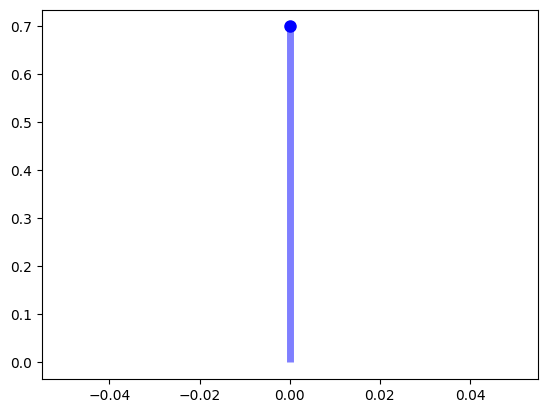
\includegraphics{figura1.png} 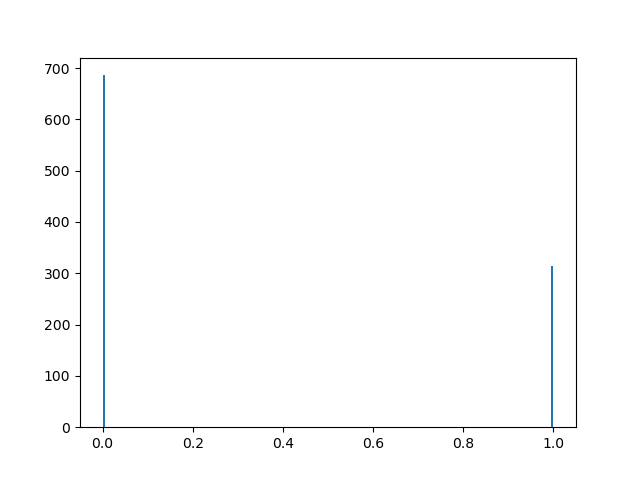
\includegraphics{F2.png}

\begin{exercise}[]\protect\hypertarget{exr-2}{}\label{exr-2}

Se generan variables aleatorias normales y el histograma de los valores
que toma.

\end{exercise}

\begin{codelisting}

\caption{\texttt{Exploring functions to generate random variables with a Gaussian distribution.py}}

\begin{Shaded}
\begin{Highlighting}[]
\ImportTok{import}\NormalTok{ numpy }\ImportTok{as}\NormalTok{ np}
\ImportTok{import}\NormalTok{ matplotlib.pyplot }\ImportTok{as}\NormalTok{ plt}
\ImportTok{from}\NormalTok{ scipy.stats }\ImportTok{import}\NormalTok{ norm}

\NormalTok{fig, ax }\OperatorTok{=}\NormalTok{ plt.subplots(}\DecValTok{1}\NormalTok{, }\DecValTok{1}\NormalTok{)}
\NormalTok{mean, var, skew, kurt }\OperatorTok{=}\NormalTok{ norm.stats(moments}\OperatorTok{=}\StringTok{\textquotesingle{}mvsk\textquotesingle{}}\NormalTok{)}

\NormalTok{x }\OperatorTok{=}\NormalTok{ np.linspace(norm.ppf(}\FloatTok{0.01}\NormalTok{), norm.ppf(}\FloatTok{0.99}\NormalTok{), }\DecValTok{100}\NormalTok{)}
\NormalTok{ax.plot(}
\NormalTok{    x,}
\NormalTok{    norm.pdf(x),}
    \StringTok{\textquotesingle{}r{-}\textquotesingle{}}\NormalTok{,}
\NormalTok{    lw}\OperatorTok{=}\DecValTok{5}\NormalTok{,}
\NormalTok{    alpha}\OperatorTok{=}\FloatTok{0.6}\NormalTok{,}
\NormalTok{    label}\OperatorTok{=}\StringTok{\textquotesingle{}norm pdf\textquotesingle{}}
\NormalTok{)}
\NormalTok{rv }\OperatorTok{=}\NormalTok{ norm()}
\NormalTok{ax.plot(x, rv.pdf(x), }\StringTok{\textquotesingle{}k{-}\textquotesingle{}}\NormalTok{, lw}\OperatorTok{=}\DecValTok{2}\NormalTok{, label}\OperatorTok{=}\StringTok{\textquotesingle{}frozen pdf\textquotesingle{}}\NormalTok{)}
\NormalTok{vals }\OperatorTok{=}\NormalTok{ norm.ppf([}\FloatTok{0.001}\NormalTok{, }\FloatTok{0.5}\NormalTok{, }\FloatTok{0.999}\NormalTok{])}

\NormalTok{np.allclose([}\FloatTok{0.001}\NormalTok{, }\FloatTok{0.5}\NormalTok{, }\FloatTok{0.999}\NormalTok{], norm.cdf(vals))}

\NormalTok{r }\OperatorTok{=}\NormalTok{ norm.rvs(size}\OperatorTok{=}\DecValTok{50000}\NormalTok{)}

\NormalTok{ax.hist(r, density}\OperatorTok{=}\VariableTok{True}\NormalTok{, bins}\OperatorTok{=}\StringTok{\textquotesingle{}auto\textquotesingle{}}\NormalTok{, histtype}\OperatorTok{=}\StringTok{\textquotesingle{}stepfilled\textquotesingle{}}\NormalTok{, alpha}\OperatorTok{=}\FloatTok{0.2}\NormalTok{)}
\NormalTok{ax.set\_xlim([x[}\DecValTok{0}\NormalTok{], x[}\OperatorTok{{-}}\DecValTok{1}\NormalTok{]])}
\NormalTok{ax.legend(loc}\OperatorTok{=}\StringTok{\textquotesingle{}best\textquotesingle{}}\NormalTok{, frameon}\OperatorTok{=}\VariableTok{False}\NormalTok{)}
\NormalTok{plt.show()}
\end{Highlighting}
\end{Shaded}

\end{codelisting}

\begin{figure}

{\centering 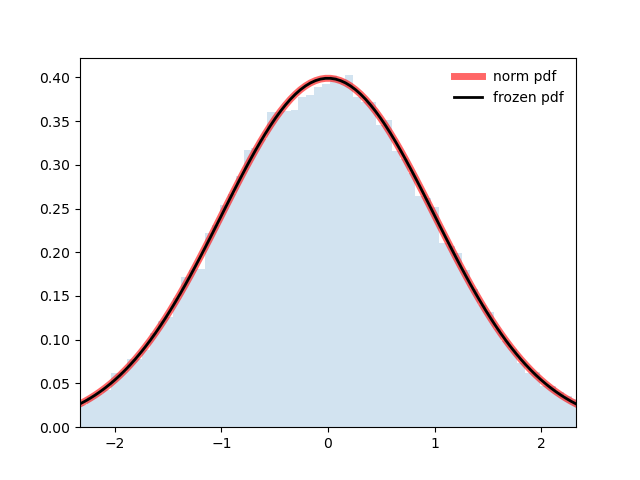
\includegraphics{Figure_3.png}

}

\caption{Figura 3}

\end{figure}

\begin{exercise}[]\protect\hypertarget{exr-3}{}\label{exr-3}

Modificando reproducir el gráfico de una distribución gaussiana
bivariada con media vectorial \(\mu[0.1, 0.5]\) y matriz de covarianza
\[\Sigma=
\begin{bmatrix}
3.0 & 0.3\\
0.75 & 1.5
\end{bmatrix}
\]

\end{exercise}

\begin{codelisting}

\caption{\texttt{Revising multivariate Gaussian.py}}

\begin{Shaded}
\begin{Highlighting}[]
\ImportTok{import}\NormalTok{ numpy }\ImportTok{as}\NormalTok{ np}
\ImportTok{import}\NormalTok{ matplotlib.pyplot }\ImportTok{as}\NormalTok{ plt}
\ImportTok{from}\NormalTok{ mpl\_toolkits.mplot3d }\ImportTok{import}\NormalTok{ axes3d}
\ImportTok{from}\NormalTok{ scipy.stats }\ImportTok{import}\NormalTok{ multivariate\_normal}

\NormalTok{x }\OperatorTok{=}\NormalTok{ np.linspace(}\DecValTok{0}\NormalTok{, }\DecValTok{5}\NormalTok{, }\DecValTok{100}\NormalTok{, endpoint}\OperatorTok{=}\VariableTok{False}\NormalTok{)}
\NormalTok{y }\OperatorTok{=}\NormalTok{ multivariate\_normal.pdf(x, mean}\OperatorTok{=}\FloatTok{2.5}\NormalTok{, cov}\OperatorTok{=}\FloatTok{0.5}\NormalTok{)}\OperatorTok{;}

\NormalTok{fig1 }\OperatorTok{=}\NormalTok{ plt.figure()}
\NormalTok{ax }\OperatorTok{=}\NormalTok{ fig1.add\_subplot(}\DecValTok{111}\NormalTok{)}
\NormalTok{ax.plot(x, y)}
\CommentTok{\# plt.show()}

\NormalTok{x, y }\OperatorTok{=}\NormalTok{ np.mgrid[}\OperatorTok{{-}}\DecValTok{5}\NormalTok{:}\DecValTok{5}\NormalTok{:}\FloatTok{.1}\NormalTok{, }\OperatorTok{{-}}\DecValTok{5}\NormalTok{:}\DecValTok{5}\NormalTok{:}\FloatTok{.1}\NormalTok{]}
\NormalTok{pos }\OperatorTok{=}\NormalTok{ np.dstack((x, y))}
\NormalTok{rv }\OperatorTok{=}\NormalTok{ multivariate\_normal([}\FloatTok{0.1}\NormalTok{, }\FloatTok{0.5}\NormalTok{], [[}\FloatTok{3.0}\NormalTok{, }\FloatTok{0.3}\NormalTok{], [}\FloatTok{0.75}\NormalTok{, }\FloatTok{1.5}\NormalTok{]])}
\NormalTok{fig2 }\OperatorTok{=}\NormalTok{ plt.figure()}
\NormalTok{ax2 }\OperatorTok{=}\NormalTok{ fig2.add\_subplot(}\DecValTok{111}\NormalTok{)}
\NormalTok{ax2.contourf(x, y, rv.pdf(pos))}
\CommentTok{\# plt.show()}

\NormalTok{ax }\OperatorTok{=}\NormalTok{ plt.figure().add\_subplot(projection}\OperatorTok{=}\StringTok{\textquotesingle{}3d\textquotesingle{}}\NormalTok{)}
\NormalTok{ax.plot\_surface(}
\NormalTok{    x,}
\NormalTok{    y,}
\NormalTok{    rv.pdf(pos),}
\NormalTok{    edgecolor}\OperatorTok{=}\StringTok{\textquotesingle{}royalblue\textquotesingle{}}\NormalTok{,}
\NormalTok{    lw}\OperatorTok{=}\FloatTok{0.5}\NormalTok{,}
\NormalTok{    rstride}\OperatorTok{=}\DecValTok{8}\NormalTok{,}
\NormalTok{    cstride}\OperatorTok{=}\DecValTok{8}\NormalTok{,}
\NormalTok{    alpha}\OperatorTok{=}\FloatTok{0.4}
\NormalTok{)}
\NormalTok{ax.contour(x, y, rv.pdf(pos), zdir}\OperatorTok{=}\StringTok{\textquotesingle{}z\textquotesingle{}}\NormalTok{, offset}\OperatorTok{={-}}\FloatTok{.2}\NormalTok{, cmap}\OperatorTok{=}\StringTok{\textquotesingle{}coolwarm\textquotesingle{}}\NormalTok{)}
\NormalTok{ax.contour(x, y, rv.pdf(pos), zdir}\OperatorTok{=}\StringTok{\textquotesingle{}x\textquotesingle{}}\NormalTok{, offset}\OperatorTok{={-}}\DecValTok{5}\NormalTok{, cmap}\OperatorTok{=}\StringTok{\textquotesingle{}coolwarm\textquotesingle{}}\NormalTok{)}
\NormalTok{ax.contour(x, y, rv.pdf(pos), zdir}\OperatorTok{=}\StringTok{\textquotesingle{}y\textquotesingle{}}\NormalTok{, offset}\OperatorTok{=}\DecValTok{5}\NormalTok{, cmap}\OperatorTok{=}\StringTok{\textquotesingle{}coolwarm\textquotesingle{}}\NormalTok{)}

\NormalTok{ax.}\BuiltInTok{set}\NormalTok{(}
\NormalTok{    xlim}\OperatorTok{=}\NormalTok{(}\OperatorTok{{-}}\DecValTok{5}\NormalTok{, }\DecValTok{5}\NormalTok{),}
\NormalTok{    ylim}\OperatorTok{=}\NormalTok{(}\OperatorTok{{-}}\DecValTok{5}\NormalTok{, }\DecValTok{5}\NormalTok{),}
\NormalTok{    zlim}\OperatorTok{=}\NormalTok{(}\OperatorTok{{-}}\FloatTok{0.2}\NormalTok{, }\FloatTok{0.2}\NormalTok{),}
\NormalTok{    xlabel}\OperatorTok{=}\StringTok{\textquotesingle{}X\textquotesingle{}}\NormalTok{,}
\NormalTok{    ylabel}\OperatorTok{=}\StringTok{\textquotesingle{}Y\textquotesingle{}}\NormalTok{,}
\NormalTok{    zlabel}\OperatorTok{=}\StringTok{\textquotesingle{}Z\textquotesingle{}}
\NormalTok{)}
\NormalTok{plt.show()}
\end{Highlighting}
\end{Shaded}

\end{codelisting}

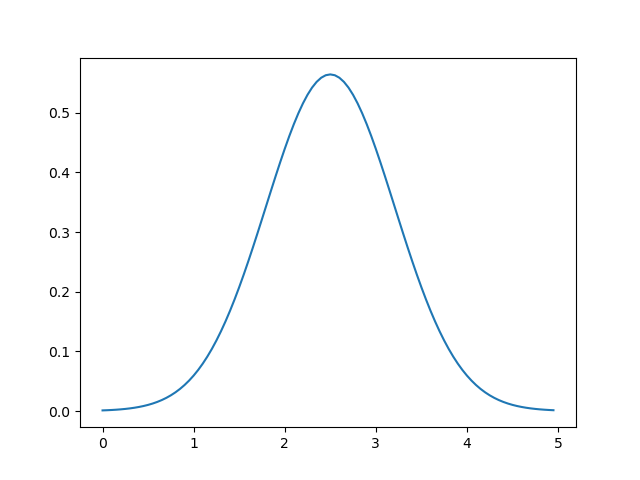
\includegraphics{Figure_4.png} 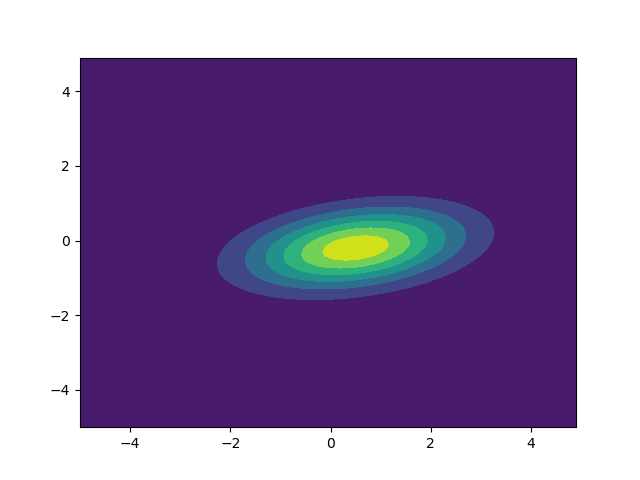
\includegraphics{Figure_5.png}
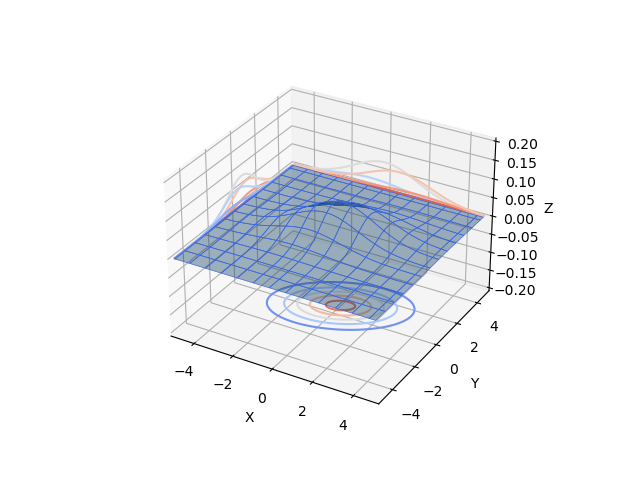
\includegraphics{Figure_6.png}

\bookmarksetup{startatroot}

\hypertarget{tarea-2}{%
\chapter{Tarea 2}\label{tarea-2}}

Sea \(Y_{\delta,h}(t)\) una caminata aleatoria. Demuestre que para
\(\delta\) y \(h\) pequeño tenemos

\[
E\exp[i\lambda Y_{\delta,h}(t)]\thickapprox\exp\left[-\frac{t\lambda^{2}h^{2}}{2\delta}-\frac{t\lambda^{4}h^{4}}{12\delta}\right]
\]

\hypertarget{demostraciuxf3n}{%
\section*{Demostración:}\label{demostraciuxf3n}}
\addcontentsline{toc}{section}{Demostración:}

\markright{Demostración:}

Considere una caminata aleatoria que comienza en 0 con saltos \(h\) y
\(-h\) igualmente probables en los momentos \(\delta\), 2
\(\delta\),\(\dots\), donde \(h\) y \(\delta\) son números positivos.
Más precisamente, sea \(\{X_{n}\}_{n=1}^{\infty}\) una sucesión de
elementos aleatorios independientes e idénticamente distribuidos.
variables con \[
P\left[X_{i}=h\right]=P\left[X_{i}=-h\right]=\dfrac{1}{2},\forall i,
\]

Sea \(Y_{\delta,h}(0)=0\) y pongamos \[
Y_{\delta,h}(n\delta)=X_{1}+X_{2}+\cdots+X_{n}.
\]

Para \(t>0\), defina \(Y_{\delta,h}(t)\) mediante linealización, es
decir, para \(n\delta<t<(n + 1)\delta\), defina \[
Y_{\delta,h}(t)=\frac{(n+1)\delta-t}{\delta}Y_{\delta,h}(n\delta)+\frac{t-n\delta}{\delta}Y_{\delta,h}((n+1)\delta).
\]

Calculemos la función característica de \(Y_{\delta,h}(t)\), donde
\(\lambda\in\mathbb{R}\) fijo y sea \(t=n\delta\) así, \(n=t/\delta\).
Entonces se tiene que

\begin{equation}\protect\hypertarget{eq-4.1}{}{
\begin{align}
    E\exp\left[i\lambda Y_{n,\delta}\left(t\right)\right] & = \prod_{j=1}^{n}Ee^{i\lambda X_{j}},\text{ por ser variables independientes,}\nonumber\\
    & = (Ee^{i\lambda X_{j}})^{n},\text{ por ser idénticamente distribuidas,}\nonumber\\
    & =  \frac{1}{2}(e^{i\lambda h}+e^{-i\lambda h})^{n},\nonumber\\
    & =  (\cos(\lambda h))^{n},\nonumber\\
    & =  (\cos(\lambda h))^{t/\delta},
\end{align}
}\label{eq-4.1}\end{equation}

Por otro lado, sea
\(u=\left[\cos\left(\lambda h\right)\right]^{1/\delta}\Rightarrow\ln\left(u\right)=\dfrac{1}{\delta}\ln\left[\cos\left(\lambda h\right)\right]\).

Usando la expansión de Taylor de \(\cos\left(x\right)\) se tiene que \[
\cos\left(\lambda h\right)\approx1-\dfrac{\left(\lambda h\right)^{2}}{2!}+\dfrac{\left(\lambda h\right)^{4}}{4!},
\]

entonces \[
\begin{eqnarray}
    \ln\left(\cos\left(\lambda h\right)\right) & \approx & \ln\left[1-\dfrac{\left(\lambda h\right)^{2}}{2}+\dfrac{\left(\lambda h\right)^{4}}{4!}\right]\nonumber\\
 & \approx & -\dfrac{\left(\lambda h\right)^{2}}{2!}+\dfrac{\left(\lambda h\right)^{4}}{4!}-\frac{1}{2}\left(-\frac{\lambda^{2}h^{2}}{2!}+\frac{\lambda^{4}h^{4}}{4!}\right)^{2}\nonumber\\
  & = & -\dfrac{\lambda^{2} h^{2}}{2!}+\dfrac{\lambda ^{4}h^{4}}{4!}-\frac{1}{2}\left(\frac{\lambda^{4}h^{4}}{4}-\frac{\lambda^{6}h^{6}}{24^{2}}+\frac{\lambda^{8}h^{8}}{24}\right)\nonumber\\
   & = & -\dfrac{\lambda^{2} h^{2}}{2}+\dfrac{\lambda^{4} h^{4}}{24}-\frac{\lambda^{4}h^{4}}{8}-\frac{\lambda^{6}h^{6}}{(2)24^{2}}+\frac{\lambda^{8}h^{8}}{48}\nonumber\\
   & = & -\dfrac{\lambda^{2} h^{2}}{2}-\dfrac{\lambda^{4} h^{4}}{12}-\frac{\lambda^{6}h^{6}}{(2)24^{2}}+\frac{\lambda^{8}h^{8}}{48}
\end{eqnarray}
\] para una \(h\) pequeña, se satisface que, \[
-\frac{\lambda^{6}h^{6}}{(2)24^{2}}+\frac{\lambda^{8}h^{8}}{48}\approx 0
\]

Por lo tanto,
\(\ln\left(\cos\left(\lambda h\right)\right)\approx -\dfrac{\lambda^{2} h^{2}}{2}-\dfrac{\lambda^{4} h^{4}}{12}\).\textbackslash{}
Así, para \(\delta\) y \(h\) pequeña, se tiene que
\(\ln u\approx \dfrac{1}{\delta}\left(-\dfrac{\lambda^{2} h^{2}}{2}-\dfrac{\lambda^{4} h^{4}}{12}\right)\).\textbackslash{}
Entonces

\[
\begin{equation}
    u\approx\exp\left[\dfrac{1}{\delta}\left(-\dfrac{\lambda^{2} h^{2}}{2}-\dfrac{\lambda^{4} h^{4}}{12}\right)\right]
\end{equation}
\] Entonces por la ecuación (Equation~\ref{eq-4.1}), \[
\begin{equation}
    E\exp\left[i\lambda Y_{n,\delta}\left(t\right)\right]\approx\exp\left[-\dfrac{t\lambda^{2} h^{2}}{2\delta}-\dfrac{t\lambda^{4} h^{4}}{12\delta}\right]
\end{equation}
\]

Calculando el limite \[
\lim_{\delta\to0}E\left[\exp\left(i\lambda Y_{n,\delta}\left(t\right)\right)\right]=\lim_{\delta\to0}\exp\left[-t\left(\left[\dfrac{h^{2}}{\delta}\right]\left(\dfrac{\lambda^{2}}{2}-\dfrac{\lambda^{4}h^{2}}{24}\right)\right)\right],
\]

Asumamos que \(\delta\to0\), \(h\to0\) pero \(h^{2}/\delta\to\infty\).
Entonces \(\lim_{\delta\to0} Y_{\delta, h}(t)\) no existe. Por otro
lado, consideremos la siguiente renormalización,

\[
\begin{eqnarray}
    E\exp\left[i\lambda Y_{n,\delta}\left(t\right)+\dfrac{th^{2}\lambda^{2}}{2\delta}\right] & = & E\left[\exp (i\lambda Y_{n,\delta}\left(t\right))\exp\left(\dfrac{th^{2}\lambda^{2}}{2\delta}\right)\right]\nonumber\\
    & = & \exp\left(\dfrac{th^{2}\lambda^{2}}{2\delta}\right)E\exp\left[ i\lambda Y_{n,\delta}\left(t\right)\right]\nonumber\\
    & \approx & \exp\left(\dfrac{th^{2}\lambda^{2}}{2\delta}\right)\exp\left[-\dfrac{t\lambda^{2} h^{2}}{2\delta}-\dfrac{t\lambda^{4} h^{4}}{12\delta}\right]\nonumber\\
    & = & \exp\left(-\dfrac{t\lambda^{4} h^{4}}{12\delta}\right)
\end{eqnarray}
\]

Así, si \(\delta,h\to0\) de tal manera que \(h^{2}/\delta\to\infty\) y
\(h^{4}/\delta\to0\), entonces \[
\lim_{\delta\to0}E\left[\exp\left(i\lambda Y_{n,\delta}\left(t\right)+\dfrac{th^{2}\lambda^{2}}{2}\right)\right]=\lim_{\delta\to0}\exp\left(\dfrac{\left(\lambda h\right)^{4}}{24\delta}\right)=1
\]

\bookmarksetup{startatroot}

\hypertarget{tarea-3}{%
\chapter{Tarea 3}\label{tarea-3}}

\begin{exercise}[Ejercicio 1:]\protect\hypertarget{exr-1}{}\label{exr-1}

Si \(X\thicksim N(\mu,\sigma^{2})\) entonces
\(\left(\dfrac{X-\mu}{\sigma}\right)\thicksim N(0,1)\).

\end{exercise}

\begin{proof}

Calculemos la función característica de la variable
\(\dfrac{X-\mu}{\sigma}\),

\begin{equation}\protect\hypertarget{eq-5.1}{}{
\begin{eqnarray}
\varphi_{\frac{X-\mu}{\sigma}}(t) & = & E\left[e^{it\left(\frac{X-\mu}{\sigma}\right)}\right]\nonumber\\
& = & E\left[e^{\left(\frac{itX}{\sigma}-\frac{it\mu}{\sigma}\right)}\right]\nonumber\\
& = & e^{-\frac{it\mu}{\sigma}}E\left[e^{\left(\frac{itX}{\sigma}\right)}\right]\nonumber\\
& = & e^{-\frac{it\mu}{\sigma}}\int_{-\infty}^{\infty}e^{\frac{itx}{\sigma}}\frac{1}{\sigma\sqrt{2\pi}}e^{-\frac{(x-\mu)^{2}}{2\sigma^{2}}}dx\nonumber\\
& = & e^{-\frac{it\mu}{\sigma}}\frac{1}{\sigma\sqrt{2\pi}}\int_{-\infty}^{\infty}e^{\frac{itx}{\sigma}}e^{-\frac{(x-\mu)^{2}}{2\sigma^{2}}}dx\nonumber\\
& = & e^{-\frac{it\mu}{\sigma}}\frac{1}{\sigma\sqrt{2\pi}}\int_{-\infty}^{\infty}e^{\frac{itx}{\sigma}-\frac{(x-\mu)^{2}}{2\sigma^{2}}}dx\nonumber\\
& = & e^{-\frac{it\mu}{\sigma}}\frac{1}{\sigma\sqrt{2\pi}}\int_{-\infty}^{\infty}e^{-\frac{1}{2}\frac{(x-\mu)^{2}-2itx\sigma}{\sigma^{2}}}dx
\end{eqnarray}
}\label{eq-5.1}\end{equation}

Observemos que, \begin{equation}\protect\hypertarget{eq-5.2}{}{
\begin{eqnarray}\label{1.2}
\frac{(x-\mu)^{2}-2itx\sigma}{\sigma^{2}} & = & \frac{x^{2}-2x\mu+\mu^{2}-2itx\sigma}{\sigma^{2}}\nonumber\\
& = & \frac{x^{2}}{\sigma^{2}}-\frac{2x\mu}{\sigma^{2}}+\frac{\mu^{2}}{\sigma^{2}}-\frac{2itx\sigma}{\sigma^{2}}\nonumber\\
& = & \frac{x^{2}}{\sigma^{2}}-\frac{2x}{\sigma}\left(\frac{\mu+it\sigma}{\sigma^{2}}\right)+\frac{\mu^{2}}{\sigma^{2}}\nonumber\\
& = & \left(\frac{x}{\sigma}-\left(\frac{\mu+it\sigma}{\sigma}\right)\right)^{2}-\left(\frac{\mu+it\sigma}{\sigma}\right)^{2}+\frac{\mu^{2}}{\sigma^{2}}\nonumber\\
& = & \left(\frac{x}{\sigma}-\left(\frac{\mu+it\sigma}{\sigma}\right)\right)^{2}-\frac{2 it\sigma\mu}{\sigma^{2}}-\frac{(it\sigma)^{2}}{\sigma^{2}}\nonumber\\
& = & \left(\frac{x}{\sigma}-\left(\frac{\mu+it\sigma}{\sigma}\right)\right)^{2}-\frac{2 it\mu}{\sigma}+t^{2}.
\end{eqnarray}
}\label{eq-5.2}\end{equation}

Sustituyendo (Equation~\ref{eq-5.2}) en (Equation~\ref{eq-5.1}), resulta

\begin{equation}\protect\hypertarget{eq-5.3}{}{
\begin{eqnarray}
\varphi_{\frac{X-\mu}{\sigma}}(t) & = & e^{-\frac{it\mu}{\sigma}}\frac{1}{\sigma\sqrt{2\pi}}\int_{-\infty}^{\infty}e^{-\frac{1}{2}\left[\left(\frac{x}{\sigma}-\left(\frac{\mu+it\sigma}{\sigma}\right)\right)^{2}-\frac{2 it\mu}{\sigma}+t^{2}\right]}dx\nonumber\\
& = & e^{-\frac{it\mu}{\sigma}}e^{\frac{it\mu}{\sigma}-\frac{t^{2}}{2}}\frac{1}{\sigma\sqrt{2\pi}}\int_{-\infty}^{\infty}e^{-\frac{1}{2}\left(\frac{x}{\sigma}-\left(\frac{\mu+it\sigma}{\sigma}\right)\right)^{2}}dx\nonumber\\
& = & e^{-\frac{t^{2}}{2}}\frac{1}{\sigma\sqrt{2\pi}}\int_{-\infty}^{\infty}e^{-\frac{1}{2}\left(\frac{x}{\sigma}-\left(\frac{\mu+it\sigma}{\sigma}\right)\right)^{2}}dx
\end{eqnarray}
}\label{eq-5.3}\end{equation}

Sea
\(u=\frac{x}{\sigma}-\left(\frac{\mu+it\sigma}{\sigma}\right)\Longrightarrow du=\frac{1}{\sigma}dx\),
sustituyendo esto en (Equation~\ref{eq-5.3}), resulta

\begin{equation}\protect\hypertarget{eq-5.4}{}{
\begin{equation}
\varphi_{\frac{X-\mu}{\sigma}}(t) = e^{-\frac{t^{2}}{2}}\frac{1}{\sqrt{2\pi}}\int_{-\infty}^{\infty}e^{-\frac{u^{2}}{2}}du
\end{equation}
}\label{eq-5.4}\end{equation}

de aquí se sigue que \(u\thicksim N(0,1)\), entonces \[
\frac{1}{\sqrt{2\pi}}\int_{-\infty}^{\infty}e^{-\frac{u^{2}}{2}}dx=1.
\] sustituyendo esto ultimo en (Equation~\ref{eq-5.4}), se tiene,

\begin{equation}\protect\hypertarget{eq-5.5}{}{
\begin{equation}
\varphi_{\frac{X-\mu}{\sigma}}(t) =e^{-\frac{t^{2}}{2}},
\end{equation}
}\label{eq-5.5}\end{equation} Por otro lado, consideremos
\(Z\thicksim N(0,1)\), entonces \[
\begin{equation*}
\varphi_{Z}(t) =e^{-\frac{t^{2}}{2}}.
\end{equation*}
\]

Entonces \(\varphi_{Z}(t)=\varphi_{\frac{X-\mu}{\sigma}}(t)\), como las
funciones características coinciden se concluye que
\(\frac{X-\mu}{\sigma}\thicksim N(0,1)\).

\end{proof}

\begin{exercise}[]\protect\hypertarget{exr-2}{}\label{exr-2}

Si \(Y\thicksim N(0,1)\) entonces
\(\sigma Y+\mu \thicksim N(\mu,\sigma)\).

\end{exercise}

\begin{proof}

Calculemos la función característica de la variable \(\sigma Y+\mu\),
\begin{equation}\protect\hypertarget{eq-5.6}{}{
\begin{eqnarray}
\varphi_{\sigma Y+\mu}(t) & = & E\left[e^{it(\sigma Y+\mu)}\right]\nonumber\\
& = & E\left[e^{it\sigma Y+it\mu}\right]\nonumber\\
& = & e^{it\mu}E\left[e^{it\sigma Y}\right]\nonumber\\
& = & e^{it\mu}\int_{-\infty}^{\infty}e^{it\sigma y}\frac{1}{\sqrt{2\pi}}e^{\frac{-y^{2}}{2}}dy\nonumber\\
& = & e^{it\mu}\frac{1}{\sqrt{2\pi}}\int_{-\infty}^{\infty}e^{-\frac{1}{2}(y^{2}-2yit\sigma) }dy.
\end{eqnarray}
}\label{eq-5.6}\end{equation}

Observemos que, \begin{equation}\protect\hypertarget{eq-5.7}{}{
\begin{eqnarray}
y^{2}-2yit\sigma & = & (y-it\sigma)^{2}-(it\sigma)^{2}\nonumber\\
& = & (y-it\sigma)^{2}+t^{2}\sigma^{2}.
\end{eqnarray}
}\label{eq-5.7}\end{equation}

Sustituyendo, (Equation~\ref{eq-5.7}) en (Equation~\ref{eq-5.6}) resulta

\begin{equation}\protect\hypertarget{eq-5.8}{}{
\begin{eqnarray}
\varphi_{\sigma Y+\mu}(t) & = & e^{it\mu}\frac{1}{\sqrt{2\pi}}\int_{-\infty}^{\infty}e^{-\frac{1}{2}((y-it\sigma)^{2}+t^{2}\sigma^{2}) }dy\nonumber\\
& = & e^{it\mu}e^{-\frac{1}{2}t^{2}\sigma^{2}}\frac{1}{\sqrt{2\pi}}\int_{-\infty}^{\infty}e^{-\frac{1}{2}(y-it\sigma)^{2} }dy
\end{eqnarray}
}\label{eq-5.8}\end{equation}

Tomando \(u=y-it\sigma\Longrightarrow du=dy\), se tiene que \[
\frac{1}{\sqrt{2\pi}}\int_{-\infty}^{\infty}e^{-\frac{1}{2}(y-it\sigma)^{2} }dy=\frac{1}{\sqrt{2\pi}}\int_{-\infty}^{\infty}e^{-\frac{u^{2} }{2}}du,
\] entonces \(U\thicksim N(0,1)\), por lo tanto, \[
\frac{1}{\sqrt{2\pi}}\int_{-\infty}^{\infty}e^{-\frac{1}{2}(y-it\sigma)^{2} }dy=1
\]

sustituyendo esto ultimo en (Equation~\ref{eq-5.8}), resulta, \[ 
\varphi_{\sigma Y+\mu}(t)=e^{it\mu}e^{-\frac{1}{2}t^{2}\sigma^{2}}=e^{it\mu-\frac{t^{2}\sigma^{2}}{2}}.
\] Sea \(Z\) una variable aleatoria tal que \(Z\thicksim N(\mu,\sigma)\)
sabemos que, \[ 
\varphi_{Z}(t)=e^{it\mu-\frac{t^{2}\sigma^{2}}{2}}.
\] De estas dos ultimas igualdades se sigue que, \[ 
\varphi_{Z}(t)=\varphi_{\sigma Y+\mu}(t).
\] Dado que tienen iguales funciones características se concluye que, \[
\sigma Y+\mu\thicksim N(\mu,\sigma)
\]

\end{proof}

\begin{exercise}[]\protect\hypertarget{exr-3}{}\label{exr-3}

Si \(X\thicksim N(\mu_{1},\sigma_{1}^{2})\),
\(Y\thicksim N(\mu_{2},\sigma_{2}^{2})\) además \(X\) y \(Y\) son
independientes entonces
\(X+Y\thicksim N(\mu_{1}+\mu_{2},\sigma_{1}^{2}+\sigma_{2}^{2})\).

\end{exercise}

\begin{proof}

Por definición, se tiene que,

\begin{equation}\protect\hypertarget{eq-5.9}{}{
\begin{eqnarray}
\varphi_{X+Y}(t) & = & E[e^{it(X+Y)}]\nonumber\\
& = & E[e^{itX}e^{itY}]\text{ por ser independientes, del ejercicio 4}\nonumber\\
& = & E[e^{itX}]E[e^{itY}]\nonumber\\
& = &  \varphi_{X}(t) \varphi_{Y}(t).
\end{eqnarray}
}\label{eq-5.9}\end{equation}

Por otro lado, sea \(Z\) una variables aleatoria tal que,
\(Z\thicksim N(\mu_{1}+\mu_{2},\sigma_{1}^{2}+\sigma_{2}^{2})\), sabemos
que la función característica de \(Z\), esta dada por,

\[
\begin{eqnarray*}
\varphi_{Z}(t) & = & e^{it(\mu_{1}+\mu_{2})-\frac{t^{2}}{2}(\sigma_{1}^{2}+\sigma_{2}^{2})}\nonumber\\
& = & e^{it\mu_{1}-\frac{t^{2}\sigma_{1}^{2}}{2}+it\mu_{2}-\frac{t^{2}\sigma_{2}^{2}}{2}}\nonumber\\
& = & e^{it\mu_{1}-\frac{t^{2}\sigma_{1}^{2}}{2}}e^{it\mu_{2}-\frac{t^{2}\sigma_{2}^{2}}{2}}\\
& = &  \varphi_{X}(t) \varphi_{Y}(t),
\end{eqnarray*}
\]

entonces, de esta ultima igualdad y de (Equation~\ref{eq-5.9}) se sigue
que, \[
\varphi_{Z}(t)= \varphi_{X+Y}(t).
\]

Como las funciones características coinciden se sigue que,
\(X+Y\thicksim N(\mu_{1}+\mu_{2},\sigma_{1}^{2}+\sigma_{2}^{2})\).

\end{proof}

\begin{exercise}[Ejercicio 4:]\protect\hypertarget{exr-4}{}\label{exr-4}

Si \(X\), \(Y\) son variables aleatorias normales entonces \(X\), \(Y\)
son independientes si y solo si \(E(XY)=E(X)E(Y)\).

\end{exercise}

\begin{proof}

Primero recordemos que \[
E\left(XY\right)=\int_{-\infty}^{\infty}\int_{-\infty}^{\infty}xyf_{XY}\left(x,y\right)\mathrm{d}x\mathrm{d}y
\]

Como \(X,Y\) son independientes, sabemos que \[
f_{XY}\left(x,y\right)=f_{X}\left(x\right)f_{Y}\left(y\right)
\]

Entonces

\[
\begin{align*}
E\left(XY\right) & =\int_{-\infty}^{\infty}\int_{-\infty}^{\infty}xyf_{XY}\left(x,y\right)\mathrm{d}x\mathrm{d}y\\
& =\int_{-\infty}^{\infty}\int_{-\infty}^{\infty}xyf_{X}\left(x\right)f_{y}\left(y\right)\mathrm{d}x\mathrm{d}y\\
& =\left(\int_{-\infty}^{\infty}xf_{X}\left(x\right)\mathrm{d}x\right)\left(\int_{-\infty}^{\infty}yf_{y}\left(y\right)\mathrm{d}y\right)\\
& =E\left(X\right)E\left(Y\right)
\end{align*}
\]

\end{proof}

\begin{theorem}[Desigualdad de
Chebyshev]\protect\hypertarget{thm-5.1}{}\label{thm-5.1}

Sea \(X\) una variable aleatoria con esperanza \(\mu=E(X)\) y sea
\(\varepsilon>0\). Entonces \[
P(|X-\mu|\geq\varepsilon)\leq\frac{Var(X)}{\varepsilon^{2}}
\]

\end{theorem}

\begin{proof}

Sea \(Y=\left|X-\mu\right|\), observemos que \(Y\) es positiva, así por
la desigualdad de Markov y dado que
\(\mathcal{P}\left[\left|X-\mu\right|\geq\epsilon\right] =\mathcal{P}\left[\left|X-\mu\right|^{2}\geq\epsilon^{2}\right]\),
se cumple que

\[
\begin{align*}
\mathcal{P}\left[\left|X-\mu\right|\geq\epsilon\right] & =\mathcal{P}\left[\left|X-\mu\right|^{2}\geq\epsilon^{2}\right]\\
& \leq\dfrac{E\left[\left(X-\mu\right)^{2}\right]}{\epsilon^{2}}=\dfrac{\text{Var}\left[X\right]}{\epsilon^{2}}
\end{align*}
\]

\end{proof}

\begin{theorem}[Ley de los grandes
números]\protect\hypertarget{thm-5.2}{}\label{thm-5.2}

Sean \(X_{1},X_{2},\dots, X_{n}\) procesos de ensayos independientes,
con esperanza finita \(\mu=E(X_{j})\) y varianza finita
\(\sigma^{2}=Var(X_{j})\). Sean \(S_{n}=X_{1}+X_{2}+\ldots+X_{n}\).
Entonces para cada \(\epsilon>0\).

\[
\mathcal{P}\left[\left|\dfrac{S_{n}}{n}-\mu\right|\geq\epsilon\right]\to0
\]

\end{theorem}

\begin{proof}

Observemos que \[
\begin{align*}
\text{Var}\left[\dfrac{S_{n}}{n}-\mu\right] & =\dfrac{1}{n^{2}}\text{Var}\left(S_{n}\right)\\
& =\dfrac{1}{n^{2}}\sum_{i=1}^{n}\text{Var}\left(X_{i}\right),\text{ por ser iid}\\
& =\dfrac{\sigma^{2}}{n}
\end{align*}
\]

Entonces, por el Teorema 5.1, \[
\mathcal{P}\left[\left|\dfrac{S_{n}}{n}-\mu\right|\geq\epsilon\right]\leq\dfrac{\sigma^{2}}{n\epsilon},
\] así, tomando el limite cuando \(n\to\infty\) \[
\dfrac{\sigma^{2}}{n\epsilon}\to0.
\]

Entonces \[
\mathcal{P}\left[\left|\dfrac{S_{n}}{n}-\mu\right|\geq\epsilon\right]\to0
\]

\end{proof}

\begin{theorem}[Teorema del Limite
Central]\protect\hypertarget{thm-5.3}{}\label{thm-5.3}

Sea \(\left\{ X_{i}\right\} _{i=1}^{\infty}\) una secuencia de v.a.i.id
con media \(a\) y varianza \(b^{2}\). Entonces para doo
\(\alpha,\beta\in\mathbb{R}\), con \(\alpha<\beta\), entonces \[
\mathcal{P}\left(\lim_{M\to\infty}\alpha\le\dfrac{{\displaystyle \sum_{i=1}^{M}}X_{i}-Ma}{\sqrt{M}b}\leq\beta\right)=\dfrac{1}{\sqrt{2\pi}}\int_{\alpha}^{\beta}e^{\left(-\dfrac{1}{2}x^{2}\right)}\mathrm{d}x
\]

\end{theorem}

\begin{proof}

Definamos a \[
S_{M}={\displaystyle \sum_{i=1}^{M}}\left[X_{i}-a\right],
\] y \[
Y_{M}=\dfrac{S_{M}}{\sqrt{M}b}.
\] Sea \(\varphi_{Y_{M}}\) la función generadora de momentos de
\(Y_{M}\) y \(\varphi\) la función generadora de momentos de la
distribución normal estándar, demostraremos que
\(\varphi_{Y_{M}}\to\varphi\).

Por definición, \[
\begin{align*}
\varphi_{Y_{M}}\left(t\right) & =E\left[\exp\left(t\dfrac{S_{M}}{\sqrt{Mb}}\right)\right]\\
& =\varphi_{S_M}\left(\dfrac{t}{\sqrt{M}b}\right)\\
& =\left[\varphi_{\left(X_{1}-a\right)}\left(\dfrac{t}{\sqrt{M}b}\right)\right]^{M} \text{ ya que, las }X_{i}\text{ son i.i.d}\\
& =\left[E\left[\exp\left(\dfrac{t}{b\sqrt{M}}\left(X_{1}-a\right)\right)\right]\right]^{M}
\end{align*}
\]

Recordando la serie de Taylor \[
\begin{align*}
\varphi_{Y_M}\left(t\right) & =\left[\sum_{i=0}^{\infty}\dfrac{E\left[\left(\dfrac{t}{b\sqrt{M}}\left(X_{1}-a\right)\right)^{i}\right]}{i!}\right]^{M}\\
& =\left[1+\dfrac{1}{2}\left(\dfrac{t}{b\sqrt{M}}\right)^{2}E\left[\left(X_{1}-a\right)^{2}\right]+\epsilon\left(3\right)\right]^{M}\\
& =\left[1+\dfrac{1}{M}\dfrac{t^{2}}{2}+\epsilon\left(3\right)\right]^{M},
\end{align*}
\]

donde \[
\begin{align*}
\epsilon\left(3\right) & =\sum_{i=3}^{\infty}\dfrac{E\left[\left(\dfrac{t}{b\sqrt{M}}\left(X_{1}-a\right)\right)^{i}\right]}{i!},
\end{align*}
\]

Ahora sea \(s=\dfrac{t}{b\sqrt{M}},\) así,\\
\[
\epsilon\left(3\right)=\sum_{i=3}^{\infty}\dfrac{E\left[\left(X_{1}-a\right)^{i}\right]s^{i}}{i!}
\] Además observemos que, cuando \(t\to0\), \(s\to0\).

Así, de lo anterior, si \(\varphi_{1}\) existe, se cumple que, \[
\dfrac{\epsilon\left(3\right)}{s^{2}}=\sum_{i=3}^{\infty}\dfrac{E\left[\left(X_{1}-a\right)^{i}\right]s^{i-2}}{i!}\to0,\text{ cuando, }s\to0.
\]

Por otro lado,

\[
\varphi_{Y_M}\left(t\right)=\left[1+\dfrac{1}{M}\left[\dfrac{t^{2}}{2}+M\epsilon\left(3\right)\right]\right]^{M},
\] y \(s\to0\) cuando \(M\to\infty\).

Entonces
\(\epsilon\left(3\right)s^{-2}=M\epsilon\left(3\right)b^{2}t^{-2}\to0\).
Dado que \(b,t\) estan fijas, se cumple que \[
M\epsilon\left(3\right)\to0,\text{ cuando, }M\to\infty,
\]

por lo tanto \[
\dfrac{t^{2}}{2}+M\epsilon\left(3\right) \to\dfrac{t^{2}}{2},\text{ cuando, }M\to\infty
\] esto implica que,

\[
\left[1+\dfrac{1}{M}\left[\dfrac{t^{2}}{2}+M\epsilon\left(3\right)\right]\right]^{M} \to\exp\left(t^{2}/2\right),M\to\infty
\]

De aqui se concluye que, \[
\lim_{M\to\infty}\varphi_{M}\left(t\right)  =\exp\left(t^{2}/2\right)=\varphi\left(t\right)
\]

la cual es la función generadora de momentos de la distribución normal
estándar. Por lo tanto \[
F_{M}\left(x\right)\to F_{N\left(0,1\right)}\left(x\right)
\] que es equivalente a,

\[
F_{M}\left(b\right)-F_{M}\left(a\right)  \to F_{N}\left(b\right)-F_{N}\left(a\right)
\] \[
\mathcal{P}\left(\lim_{M\to\infty}\alpha\le\dfrac{{\displaystyle \sum_{i=1}^{M}}X_{i}-Ma}{\sqrt{M}b}\leq\beta\right) =\dfrac{1}{\sqrt{2\pi}}\int_{\alpha}^{\beta}\exp\left(-\dfrac{1}{2}x^{2}\right)\mathrm{d}x
\]

\end{proof}

\begin{theorem}[]\protect\hypertarget{thm-5.4}{}\label{thm-5.4}

Sea \(\left\{ X_{i}\right\} _{i=1}^{\infty}\) una sucesión de v.a.i.i.d
con media \(a\). Entonces \[
\mathcal{P}\left[\lim_{M\to\infty}\dfrac{1}{M}\sum_{i=1}^{M}X_{i}=a\right]=1.
\]

\end{theorem}

\begin{proof}

Esto es similar a decir que \[
\lim_{M\to\infty}\dfrac{1}{M}\sum_{i=1}^{M}X_{i}\stackrel{\text{c.s}}{=}a
\]

Sin perdida de generalidad, diremos que \(X_{i}\geq0,\forall i\).
Definamos \[
Y_{n}=X_{n}I_{\left[\left|X_{n}\right|\leq n\right]},Q_{n}=\sum_{i=1}^{n}Y_{i}
\]

Por la desigualdad de \[
\begin{align*}
\sum_{n=1}^{\infty}\mathcal{P}\left[\left|\dfrac{Q_{n}-E\left[Q_{n}\right]}{n}\right|\geq\epsilon\right] & \leq\sum_{n=1}^{\infty}\dfrac{\text{Var}\left(Q_{n}\right)}{\epsilon^{2}n^{2}}=\sum_{n=1}^{\infty}\dfrac{1}{\epsilon^{2}n^{2}}\sum_{i=1}^{n}\text{Var}\left(Y_{i}\right)\\
& \leq\sum_{n=1}^{\infty}\dfrac{E\left(Y_{n}^{2}\right)}{\epsilon^{2}n^{2}}=\sum_{n=1}^{\infty}\dfrac{1}{\epsilon^{2}n^{2}}\int_{0}^{n}x^{2}\mathrm{d}F\\
& \leq\sum_{n=1}^{\infty}\dfrac{1}{\epsilon^{2}}\int_{0}^{n}x\mathrm{d}F<\infty,
\end{align*}
\]

donde \(F\) es la función de distribución de \(X_{i}\). Luego \[
E\left[X_{1}\right]=\lim_{n\to\infty}\int_{0}^{n}x\mathrm{d}F=\lim_{n\to\infty}E\left[Y_{n}\right]=\lim_{n\to\infty}\dfrac{E\left[Q_{n}\right]}{n}.
\]

Entonces, por el Lema de Borel Canteli.
\(\mathcal{\mathcal{P}}\left[\limsup\left(\left|\dfrac{Q_{n}-E\left[Q_{n}\right]}{n}\right|\geq\epsilon\right)\right]=0\)

\[
\lim_{n\to\infty}\dfrac{Q_{n}}{n}=E\left[X_{1}\right],\text{c.s}
\]

Ahora, calcularemos la siguiente probabilidad \[
\sum_{i=1}^{\infty}\mathcal{P}\left[X_{i}\neq Y_{i}\right]=\sum_{i=1}^{\infty}\mathcal{P}\left[X_{i}>n\right]
\]

como \(E\left[X_{i}\right]<\infty\) y \(X_{i}\) son v.a.i.i.d.

\[
\sum_{i=1}^{\infty}\mathcal{P}\left[X_{i}>n\right]\leq E\left[X_{1}\right]<\infty
\]

De nuevo, por el Lema de Borel Cantelli. \[
\mathcal{P}\left[\limsup\left[X_{i}\neq Y_{i}\right]\right]=0,\forall i
\]

Entonces \[
\begin{align*}
X_{i} & =Y_{i},\text{c.s}\\
\Rightarrow & \dfrac{1}{M}\sum_{i=1}^{M}X_{i}\to E\left[X_{1}\right]=\mu.\text{ c.s}
\end{align*}
\]

\end{proof}

\bookmarksetup{startatroot}

\hypertarget{tarea-4}{%
\chapter{Tarea 4}\label{tarea-4}}

\hypertarget{ejercicio-1-1}{%
\section{Ejercicio 1}\label{ejercicio-1-1}}

Sea \(W(t)\) un movimiento Browniano estándar en \([0,T]\). Pruebe que
para cualquier \(c>0\) fijo, \[
V(t) = \dfrac{1}{c} W(c^2 t)
\]

es un movimiento Browniano sobre \([0,T]\).

\hypertarget{demostraciuxf3n-1}{%
\subsection{Demostración}\label{demostraciuxf3n-1}}

Veamos que \(V\) cumple las propiedades del movimiento Browniano.

\hypertarget{propiedad-1-que-comience-en-0}{%
\subsubsection{Propiedad 1 (Que comience en
0)}\label{propiedad-1-que-comience-en-0}}

Se tiene que, \(V(0) = \dfrac{1}{c} W (c^2\cdot0)=0\).

\hypertarget{propiedad-2-incrementos-independientes}{%
\subsubsection{Propiedad 2 (Incrementos
Independientes)}\label{propiedad-2-incrementos-independientes}}

Sean \(s<t<u<v\), por definición de \(V\), se tiene que, \[
E[\left(V(t)-V(s)\right)\left(V(v)-V(u)\right)]=\dfrac{1}{c^2}E[\left(W(c^2 t)-W(c^2 s)\right)\left(W(c^2 v)-W(c^2 u)\right)]
\]

Dado que \(W\) tiene incrementos independientes, se cumple que.
\begin{align*}
\dfrac{1}{c^{2}}E\left[\left(W(c^{2}t)-W(c^{2}s)\right)\left(W(c^{2}v)-W(c^{2}u)\right)\right] & =\dfrac{1}{c^{2}}E\left[\left(W(c^{2}t)-W(c^{2}s)\right)\right]E\left[\left(W(c^{2}v)-W(c^{2}u)\right)\right]
\end{align*}

Entonces \(V\) tiene incrementos independientes.

\hypertarget{propiedad-3-incrementos-estacionarios}{%
\subsubsection{Propiedad 3 (Incrementos
estacionarios)}\label{propiedad-3-incrementos-estacionarios}}

Sea \(s<t\). \[
V(t)-V(s)=\dfrac{1}{c}\left[W(c^2 t) - W(c^2 s)\right]
\]

Por las propiedades de la definicion del movimiento Browniano.

\begin{align*}
E\left[V(t)-V(s)\right] & =\dfrac{1}{c}E\left[W(c^{2}t)-W(c^{2}s)\right]=0\\
\text{Var}\left[V(t)-V(s)\right] & =\dfrac{1}{c^{2}}\text{Var}\left[W(c^{2}t)-W(c^{2}s)\right]=\dfrac{1}{c^{2}}\left(c^{2}\left(t-s\right)\right)=t-s
\end{align*}

Entonces \(V\) tiene incrementos estacionarios.

Con todo lo anterior se concluye que, \(V\) es un movimiento browniano.

\hypertarget{ejercicio-2}{%
\section{Ejercicio 2}\label{ejercicio-2}}

Hacer un script para ilustrar la propiedad de escalado del movimiento
Browniano para el caso de \(c = \dfrac{1}{5}\). Estar seguro que usa el
mismo camino browniano discretizado en cada subplot.

\begin{codelisting}

\caption{\texttt{Browniano escalado, con c=1/5.py}}

\begin{Shaded}
\begin{Highlighting}[]
\ImportTok{import}\NormalTok{ numpy }\ImportTok{as}\NormalTok{ np}
\ImportTok{import}\NormalTok{ matplotlib.pyplot }\ImportTok{as}\NormalTok{ plt}
\NormalTok{prng }\OperatorTok{=}\NormalTok{ np.random.RandomState(}\DecValTok{123456789}\NormalTok{)}
\NormalTok{T }\OperatorTok{=} \DecValTok{1}  
\NormalTok{n}\OperatorTok{=} \DecValTok{100}  
\NormalTok{dt }\OperatorTok{=} \DecValTok{1} \OperatorTok{/}\NormalTok{ (n }\OperatorTok{{-}} \DecValTok{1}\NormalTok{)}
\NormalTok{dw }\OperatorTok{=}\NormalTok{ np.sqrt(dt) }\OperatorTok{*}\NormalTok{ prng.standard\_normal(n }\OperatorTok{{-}} \DecValTok{1}\NormalTok{) }
\NormalTok{w }\OperatorTok{=}\NormalTok{ np.concatenate(([}\DecValTok{0}\NormalTok{],dw.cumsum()))}

\NormalTok{time }\OperatorTok{=}\NormalTok{ np.linspace(}\DecValTok{0}\NormalTok{,T, n)}
\NormalTok{c }\OperatorTok{=} \FloatTok{0.2}  \CommentTok{\# 1/5}
\NormalTok{c\_time }\OperatorTok{=}\NormalTok{ c}\OperatorTok{**}\DecValTok{2} \OperatorTok{*}\NormalTok{ time  }
\NormalTok{c\_w }\OperatorTok{=}\NormalTok{ c}\OperatorTok{**}\NormalTok{(}\OperatorTok{{-}}\DecValTok{1}\NormalTok{) }\OperatorTok{*}\NormalTok{ w  }

\NormalTok{fig, browniano\_escalado }\OperatorTok{=}\NormalTok{ plt.subplots(}\DecValTok{2}\NormalTok{)}
\NormalTok{browniano\_escalado[}\DecValTok{0}\NormalTok{].plot(time, w)}
\NormalTok{browniano\_escalado[}\DecValTok{1}\NormalTok{].plot(c\_time, c\_w)}
\NormalTok{browniano\_escalado[}\DecValTok{0}\NormalTok{].set\_title(}\StringTok{\textquotesingle{}Movimiento browniano\textquotesingle{}}\NormalTok{)}
\NormalTok{browniano\_escalado[}\DecValTok{1}\NormalTok{].set\_title(}\StringTok{\textquotesingle{}Moviemiento browniano escalado\textquotesingle{}}\NormalTok{)}
\NormalTok{plt.show()}
\end{Highlighting}
\end{Shaded}

\end{codelisting}

\begin{figure}

{\centering 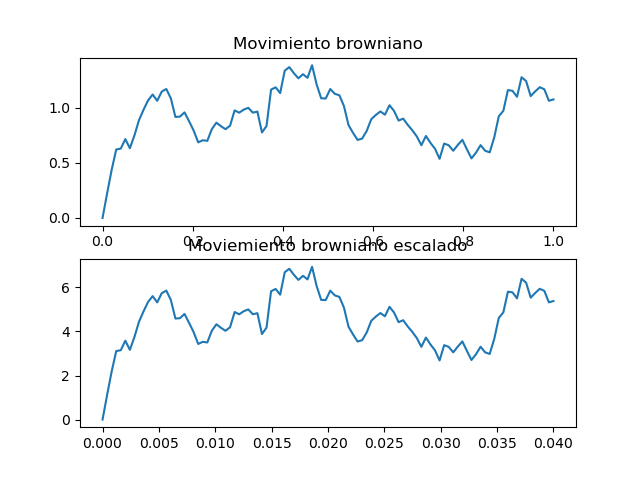
\includegraphics{Figure_T4-1.png}

}

\caption{Figura 1}

\end{figure}

\hypertarget{ejercicio-3}{%
\section{Ejercicio 3}\label{ejercicio-3}}

Modifique el script \texttt{half\_brownian\_refinement.py} encapsulando
el código en una función. Esta función deberá recibir el extremo derecho
del intervalo \([0, T]\) y el número de incrementos \(N\) de un camino
browniano base. El propósito es calcular los incrementos de relleno de
una refinamiento con \(2N\) incrementos.

\begin{codelisting}

\caption{\texttt{Browniano refinado, con refinamiento 2N.py}}

\begin{Shaded}
\begin{Highlighting}[]
\ImportTok{import}\NormalTok{ numpy }\ImportTok{as}\NormalTok{ np}
\ImportTok{import}\NormalTok{ matplotlib.pyplot }\ImportTok{as}\NormalTok{ plt}
\NormalTok{prng }\OperatorTok{=}\NormalTok{ np.random.RandomState(}\DecValTok{123456789}\NormalTok{)}

\KeywordTok{def}\NormalTok{ refined\_brownian\_2n(T,L):}
\NormalTok{    dt }\OperatorTok{=}\NormalTok{ T }\OperatorTok{/}\NormalTok{ L}
\NormalTok{    W }\OperatorTok{=}\NormalTok{ np.zeros(L }\OperatorTok{+} \DecValTok{1}\NormalTok{)}
\NormalTok{    W\_refined }\OperatorTok{=}\NormalTok{ np.zeros(}\DecValTok{2} \OperatorTok{*}\NormalTok{ L }\OperatorTok{+} \DecValTok{1}\NormalTok{)}
\NormalTok{    xi }\OperatorTok{=}\NormalTok{ np.sqrt(dt) }\OperatorTok{*}\NormalTok{ prng.normal(size}\OperatorTok{=}\NormalTok{L)}
\NormalTok{    xi\_half }\OperatorTok{=}\NormalTok{ np.sqrt(}\FloatTok{0.5} \OperatorTok{*}\NormalTok{ dt) }\OperatorTok{*}\NormalTok{ prng.normal(size}\OperatorTok{=}\NormalTok{L)}
\NormalTok{    W[}\DecValTok{1}\NormalTok{:] }\OperatorTok{=}\NormalTok{ xi.cumsum()}
\NormalTok{    W\_ }\OperatorTok{=}\NormalTok{ np.roll(W, }\OperatorTok{{-}}\DecValTok{1}\NormalTok{)}
\NormalTok{    W\_half }\OperatorTok{=} \FloatTok{0.5} \OperatorTok{*}\NormalTok{ (W }\OperatorTok{+}\NormalTok{ W\_)}
\NormalTok{    W\_half }\OperatorTok{=}\NormalTok{ np.delete(W\_half, }\OperatorTok{{-}}\DecValTok{1}\NormalTok{) }\OperatorTok{+}\NormalTok{ xi\_half}
\NormalTok{    W\_refined[}\DecValTok{1}\NormalTok{::}\DecValTok{2}\NormalTok{] }\OperatorTok{=}\NormalTok{ W\_half}
\NormalTok{    W\_refined[}\DecValTok{2}\NormalTok{::}\DecValTok{2}\NormalTok{] }\OperatorTok{=}\NormalTok{ W[}\DecValTok{1}\NormalTok{:]}
\NormalTok{    t }\OperatorTok{=}\NormalTok{ np.arange(}\DecValTok{0}\NormalTok{, T }\OperatorTok{+}\NormalTok{ dt, dt)}
\NormalTok{    t\_half }\OperatorTok{=}\NormalTok{ np.arange(}\DecValTok{0}\NormalTok{, T }\OperatorTok{+} \FloatTok{0.5} \OperatorTok{*}\NormalTok{ dt, }\FloatTok{0.5} \OperatorTok{*}\NormalTok{ dt)}
    \ControlFlowTok{return}\NormalTok{ t,t\_half,W, W\_refined}
\end{Highlighting}
\end{Shaded}

\end{codelisting}

\hypertarget{ejercicio-4-1}{%
\section{Ejercicio 4}\label{ejercicio-4-1}}

En un script separado, incluya la función de arriba y grafique una
figura con la trayectoria del browniano con 100 incrementos y muestre su
refinamiento correspondiente.

\begin{codelisting}

\caption{\texttt{Browniano refinado, con refinamiento 2N y 100 incrementos.py}}

\begin{Shaded}
\begin{Highlighting}[]
\ImportTok{import}\NormalTok{ numpy }\ImportTok{as}\NormalTok{ np}
\ImportTok{import}\NormalTok{ matplotlib.pyplot }\ImportTok{as}\NormalTok{ plt}
\ImportTok{import}\NormalTok{ h\_b\_r }\ImportTok{as}\NormalTok{ hbr}

\NormalTok{a, b, c, d }\OperatorTok{=}\NormalTok{ hbr.refined\_brownian\_2n(}\DecValTok{1}\NormalTok{, }\DecValTok{100}\NormalTok{)}

\NormalTok{plt.plot(a, c, }\StringTok{\textquotesingle{}r{-}+\textquotesingle{}}\NormalTok{)}
\NormalTok{plt.plot(}
\NormalTok{    b,}
\NormalTok{    d,}
    \StringTok{\textquotesingle{}g*{-}{-}\textquotesingle{}}\NormalTok{,}
    \CommentTok{\# alpha = transparecia}
\NormalTok{    )}
\NormalTok{plt.show()}
\end{Highlighting}
\end{Shaded}

\end{codelisting}

\begin{figure}

{\centering 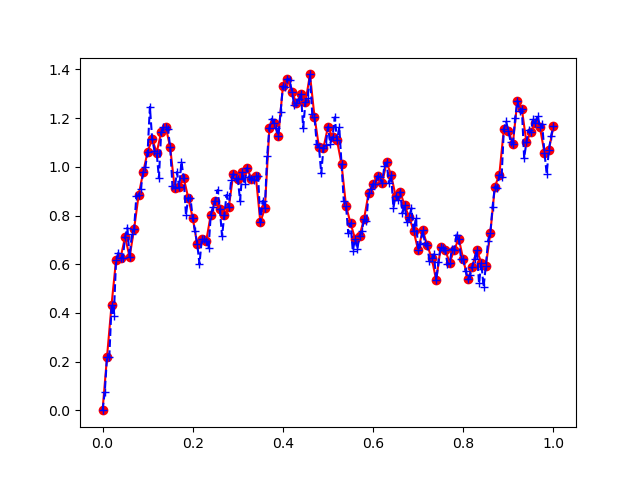
\includegraphics{Figure_2_T4.png}

}

\caption{Figura 2}

\end{figure}

\bookmarksetup{startatroot}

\hypertarget{tarea-5}{%
\chapter{Tarea 5}\label{tarea-5}}

\begin{exercise}[]\protect\hypertarget{exr-1}{}\label{exr-1}

Demuestre que el movimiento browniano satisface \[
E[|W(t)-W(s)|^{2}]=|t-s|.
\]

\end{exercise}

\begin{proof}

Consideremos dos casos:\\
Si \(t>s\). \[
\begin{align*}
E\left[\left|W\left(t\right)-W\left(s\right)\right|^{2}\right] & =E\left[\left(W\left(t\right)-W\left(s\right)\right)^{2}\right]\\
 & =t-s,
\end{align*}
\] ya que, \(W(t)-W(s)\thicksim N(0,t-s)\).\\
Mientras que si \(t\leq s\). \[
\begin{align*}
E\left[\left(W\left(t\right)-W\left(s\right)\right)^{2}\right] & =E\left[\left(W\left(s\right)-W\left(t\right)\right)^{2}\right]\\
 & =s-t,
\end{align*}
\]

por lo tanto \[
E\left[\left|W\left(t\right)-W\left(s\right)\right|^{2}\right]=\left|t-s\right|
\]

\end{proof}

\begin{exercise}[]\protect\hypertarget{exr-2}{}\label{exr-2}

Dados \(W(t_{i})\) y \(W(t_{i+1})\), demuestre que la variable aleatoria
\[
W(t_{i+\frac{1}{2}}):=\frac{1}{2}(W(t_{i})+W(t_{i+1}))+\frac{1}{2}\sqrt{\delta t\xi},\quad\xi\thicksim N(0,1)
\] satisface las tres condiciones C1, C2, C3 de la definicion de
movimiento Browniano.

\end{exercise}

\begin{proof}

(C1) Veamos que \(W\left(0\right)=0\), cuando \(t=0\).\\
Se tiene por definicion del proceso que, \[
W\left(0\right)=\frac{1}{2}(W(0)+W(0))+\frac{1}{2}\sqrt{\delta(0)\xi}=0.
\] Por la propiedad C1 se satisface.\\
\strut \\
(C2) Que tenga incrementos estacionarios.\\
Notemos que \[
\begin{align*}
W(t_{i+\frac{1}{2}})-W(t_{i}) & = \dfrac{1}{2}\left[W\left(t_{i+1}\right)+W\left(t_{i}\right)\right]+\dfrac{1}{2}\sqrt{\delta t}\xi-\frac{1}{2}(W(t_{i})+W(t_{i}))\\
& = \dfrac{1}{2}\left[W\left(t_{i+1}\right)-W\left(t_{i}\right)\right]+\dfrac{1}{2}\sqrt{\delta t}\xi,
\end{align*}
\] Entonces \[
\begin{eqnarray*}
E\left[W(t_{i+\frac{1}{2}})-W(t_{i})\right] & = & E\left[\dfrac{1}{2}\left[W\left(t_{i+1}\right)-W\left(t_{i}\right)\right]+\dfrac{1}{2}\sqrt{\delta t}\xi\right]\\
& = & E\left[\dfrac{1}{2}\left[W\left(t_{i+1}\right)-W\left(t_{i}\right)\right]\right]+E\left[\dfrac{1}{2}\sqrt{\delta t}\xi\right]\\
& = & \dfrac{1}{2}E\left[W\left(t_{i+1}\right)-W\left(t_{i}\right)\right]+\dfrac{1}{2}\sqrt{\delta t}E\left[\xi\right]\\
& = & 0\quad\text{ya que, }E\left[\xi\right]=0\text{ y }E\left[W\left(t_{i+1}\right)-W\left(t_{i}\right)\right]=0.
\end{eqnarray*}
\] y \[
\begin{eqnarray}
Var\left[W(t_{i+\frac{1}{2}})-W(t_{i})\right]& = & Var\left[\dfrac{1}{2}\left[W\left(t_{i+1}\right)-W\left(t_{i}\right)\right]+\dfrac{1}{2}\sqrt{\delta t}\xi\right]\\
& = & Var\left[\dfrac{1}{2}\left[W\left(t_{i+1}\right)-W\left(t_{i}\right)\right]\right]+Var\left[\dfrac{1}{2}\sqrt{\delta t}\xi\right]\\
& = & \dfrac{1}{4}Var\left[W\left(t_{i+1}\right)-W\left(t_{i}\right)\right]+\dfrac{1}{4}\delta t Var\left[\xi\right]\\
& = & \dfrac{1}{4}\delta t+\dfrac{1}{4}\delta t\quad\text{ya que, }Var\left[\xi\right]=1\text{ y }Var\left[W\left(t_{i+1}\right)-W\left(t_{i}\right)\right]=\delta t\\
& = & \dfrac{1}{2}\delta t.
\end{eqnarray}
\]

Además, sabemos que la combinación lineal de normales es una
nornal.\textbackslash{} Por lo tanto
\(W(t_{i+\frac{i}{2}})-W(t_{i})\sim N\left(0,\dfrac{\delta t}{2}\right)\),
con esto C2 se cumple.\\
\strut \\
(C3) Que tenga incrementos independientes.\\
Para esta parte usaremos que dos variables aleatorias \(X\) y \(Y\) son
independientes si y solo si \[ 
E(XY)=E(X)E(Y)
\]

calculemos \$
E\left[\left(W\left(t_{i+1}\right)-W\left(t_{i+\frac{1}{2}}\right)\right)\left(W(t_{j+1})-W\left(t_{j+\frac{1}{2}}\right)\right)\right]\$
y definamos a \(\Delta W(t_{i}):=W(t_{i+1})-W(t_{i})\).\\
Por lo anterior se tiene que: \[
\begin{eqnarray*}
    E\left[\left(\Delta W\left(t_{i+\frac{1}{2}}\right)\right)\left(\Delta W\left(t_{j+\frac{1}{2}}\right)\right)\right]& = & E\left[\left(\dfrac{1}{2}\Delta W\left(t_{i}\right)+\frac{1}{2}\sqrt{\delta t}\xi\right)\left(\dfrac{1}{2}\Delta W\left(t_{j}\right)+\frac{1}{2}\sqrt{\delta t}\xi\right)\right],
\end{eqnarray*}
\] donde
\(\Delta W\left(t_{i+\frac{1}{2}}\right)=W(t_{i+1})-W\left(t_{i+\frac{1}{2}}\right)\)
y
\(\Delta W\left(t_{j+\frac{1}{2}}\right)=W(t_{j+1})-W\left(t_{j+\frac{1}{2}}\right)\).\textbackslash{}
Desarrollando la parte derecha de la igualdad anterior, resulta \[
\begin{eqnarray*}
E\left[\left(\Delta W(t_{i+\frac{1}{2}})\right)\left(\Delta W(t_{j+\frac{1}{2}})\right)\right]& = & E\left[\dfrac{1}{4}\Delta W(t_{i})\Delta W(t_{j})+\dfrac{1}{4}\Delta W(t_{i})\sqrt{\delta t}\xi\right.\\
& & \left.+\dfrac{1}{4}\Delta W(t_{j})\sqrt{\delta t}\xi+\left(\frac{1}{2}\sqrt{\delta t}\xi\right)^{2}\right]\\
\text{ya que, }\Delta W(t_{i}),\Delta W(t_{j})\text{ son independientes} & = & \dfrac{1}{4}E\left[\Delta W(t_{i})\right]E\left[\Delta W(t_{j})\right]+\dfrac{1}{4}E\left[\Delta W(t_{i})\right]\sqrt{\delta t}E\left[\xi\right]+\dfrac{1}{4}E\left[\Delta W(t_{j})\right]\sqrt{\delta t}E\left[\xi\right]+\dfrac{\delta t}{4}\left(E\left[\xi\right]\right)^{2}\\
  & = & E\left[\dfrac{1}{2}\Delta W(t_{i})\right]E\left[\dfrac{1}{2}\Delta W(t_{j})+\frac{1}{2}\sqrt{\delta t}\xi\right]+E\left[\dfrac{1}{2}\Delta W(t_{j})\right]\frac{1}{2}\sqrt{\delta t}E\left[\xi\right]+\dfrac{\delta t}{4}\left(E\left[\xi\right]\right)^{2}\\
  & = & E\left[\dfrac{1}{2}\Delta W(t_{i})\right]E\left[\Delta W(t_{j+\frac{1}{2}})\right]+E\left[\dfrac{1}{2}\Delta W(t_{j})\right]\frac{1}{2}\sqrt{\delta t}E\left[\xi\right]+\dfrac{\delta t}{4}\left(E\left[\xi\right]\right)^{2}\\
 & = & E\left[\dfrac{1}{2}\Delta W(t_{i})\right]E\left[\Delta W(t_{j+\frac{1}{2}})\right] +E\left[\dfrac{1}{2}\Delta W(t_{j})+\frac{1}{2}\sqrt{\delta t}\xi\right]\frac{1}{2}\sqrt{\delta t}E\left[\xi\right]\\
 & = & E\left[\dfrac{1}{2}\Delta W(t_{i})\right]E\left[\Delta W(t_{j+\frac{1}{2}})\right]+E\left[\Delta W(t_{j+\frac{1}{2}})\right]\frac{1}{2}\sqrt{\delta t}E\left[\xi\right]\\
 & = & E\left[\dfrac{1}{2}\Delta W(t_{i})+\frac{1}{2}\sqrt{\delta t}\xi\right]E\left[\Delta W(t_{j+\frac{1}{2}})\right]\\
 & = & E\left[\Delta W(t_{i+\frac{1}{2}})\right]E\left[\Delta W(t_{j+\frac{1}{2}})\right].
\end{eqnarray*}
\]

Por lo tanto
\(E\left[\left(\Delta W(t_{i+\frac{1}{2}})\right)\left(\Delta W(t_{j+\frac{1}{2}})\right)\right]= E\left[\Delta W(t_{i+\frac{1}{2}})\right]E\left[\Delta W(t_{j+\frac{1}{2}})\right]\),
con lo que se concluye que se satisface la propiedad C3. Con todo lo
anterior se concluye que \(W(t_{i+\frac{1}{2}})\) define un Movimiento
Browniano.

\end{proof}

\begin{exercise}[]\protect\hypertarget{exr-3}{}\label{exr-3}

Generalice la formula en el \{Exercise~\ref{exr-2}\} para el caso, dado
\(W(t_{i}), W(t_{i+1})\), y \(\alpha\in(0,1)\) el valor \[
W(t_{i}+\alpha dt)
\] satisface las tres condiciones que define un movimiento Browniano.

\end{exercise}

\begin{proof}

Observemos que \[
t_{i+\alpha}=\alpha t_{i+1}+(1-\alpha)t_{i},
\] y \[
W(t_{i+\alpha})-W(t_{i}) \sim \alpha\sqrt{ dt}N(0,1)
\] Definamos a \[
W(t_{i+\alpha})=W\left(t_{i}+\alpha\Delta t\right) :=\left(1-\alpha\right)W(t_{i})+\alpha W(t_{i+1})+Y.
\] donde \(Y\) será una v.a independiente de \(W\left(t\right)\).\\
Dado que, \[
\begin{align*}
W(t_{i+\alpha})-W(t_{i}) & =\left(1-\alpha\right)W(t_{i})+\alpha W(t_{i+1})+Y-W_{i}\\
 & =\alpha\left(W_{i+1}-W(t_{i})\right)+Y.
\end{align*}
\] Entonces, \[
E\left[W(t_{i+\alpha})-W(t_{i})\right]-E[\alpha\left(W(t_{i+1})-W(t_{i})\right)]=E\left[Y\right]\Longrightarrow E[Y]=0,
\] y \[
Var\left[W(t_{i+\alpha})-W(t_{i})\right]=\alpha^{2}d t+Var\left[Y\right],
\] Así, \[
Var\left[Y\right]=d t\left(\alpha-\alpha^{2}\right),
\] entonces
\(Y=\sqrt{\alpha\left(1-\alpha\right)dt}\xi,\xi\sim N\left(0,1\right)\).\\
Con esto se cumple \(C1\). \[
W\left(0\right)=0.
\] y por construcción análogamente que el ejercicio anterior se
satisfacen las propiedades C2 y C3.

\end{proof}

\begin{exercise}[]\protect\hypertarget{exr-4}{}\label{exr-4}

Suponga que \(X\thicksim N(0,1)\), sabemos que \(E[X]=0\) y
\(E(X^{2})=1\).\\
Además de la definción, el pésimo-momento satisface \[
E[X^{p}]=\frac{1}{\pi}\int_{-\infty}^{\infty}x^{p}\exp(-x^{2}/2)dx.
\] Usando esta relación, demuestre que \(E[X^{3}]=0\) y \(E[X^{4}]=3\).
Entonces deduce que un incremento Browniano
\(\delta W_{i}:=W(t_{i+1})-W(t_{i})\) satisface que
\(E[\delta Wt_{i}^{3}]=0\) y \(E[\delta Wt_{i}^{4}]=3\delta t^{2}\).
Entonces encuentre una expresion para \(E[X^{p}]\) para un entero
positivo \(p\)

\end{exercise}

\begin{proof}

De la definición del \(p\)-esimo momento se tiene para \(p=4\), que \[
E\left[X^{4}\right]=\dfrac{1}{\sqrt{2\pi}}\int_{-\infty}^{\infty}x^{4}\exp\left(-\frac{x^{2}}{2}\right)d x.
\] resolviendo esta integral por el método integración por partes, se
tiene que \(E\left[X^{4}\right]=uv-\int vdu\) , donde
\(u=x^{3}\Longrightarrow du=3x^{2}dx\) y
\(dv=x\dfrac{1}{\sqrt{2\pi}}\exp{\left(-\dfrac{x^{2}}{2}\right)}dx\),
calculemos primero \(v\), \[
\begin{eqnarray*}
v & = & \int x\dfrac{1}{\sqrt{2\pi}}\exp{\left(-\dfrac{x^{2}}{2}\right)}dx\\
& = & \dfrac{1}{\sqrt{2\pi}}\int x\exp{\left(-\dfrac{x^{2}}{2}\right)}dx\quad\text{ sea } y=-\dfrac{x^{2}}{2}\Longrightarrow dy=-xdx\\
& = & -\dfrac{1}{\sqrt{2\pi}}\int \exp{\left(y\right)}dy\\
& = & -\dfrac{1}{\sqrt{2\pi}} \exp{\left(y\right)}\\
& = &  -\dfrac{1}{\sqrt{2\pi}}\exp{\left(-\dfrac{x^{2}}{2}\right)}.
\end{eqnarray*}
\] Sustituyendo todo lo anterior se tiene que, \[
\begin{eqnarray*}
    E\left[X^{4}\right] & = & \left.-x^{3}\dfrac{1}{\sqrt{2\pi}}\exp{\left(-\dfrac{x^{2}}{2}\right)}\right|_{-\infty}^{\infty}-\int_{-\infty}^{\infty} -\dfrac{1}{\sqrt{2\pi}}\exp{\left(-\dfrac{x^{2}}{2}\right)}3x^{2}dx\\
     & = & \left.-x^{3}\dfrac{1}{\sqrt{2\pi}}\exp{\left(-\dfrac{x^{2}}{2}\right)}\right|_{-\infty}^{\infty}+3\dfrac{1}{\sqrt{2\pi}}\int_{-\infty}^{\infty} x^{2}\exp{\left(-\dfrac{x^{2}}{2}\right)}dx\\
     & = & \left.-x^{3}\dfrac{1}{\sqrt{2\pi}}\exp{\left(-\dfrac{x^{2}}{2}\right)}\right|_{-\infty}^{\infty}+3E[X^{2}],
\end{eqnarray*}
\] por otro lado, \[
\left.-x^{3}\dfrac{1}{\sqrt{2\pi}}\exp{\left(-\dfrac{x^{2}}{2}\right)}\right|_{-\infty}^{\infty}=\lim_{x\to\infty}-x^{3}\dfrac{1}{\sqrt{2\pi}}\exp{\left(-\dfrac{x^{2}}{2}\right)}+\lim_{x\to-\infty}x^{3}\dfrac{1}{\sqrt{2\pi}}\exp{\left(-\dfrac{x^{2}}{2}\right)}=0.
\] Por lo tanto, dado que \(E[X^{2}]=1\), se concluye que \[ 
E\left[X^{4}\right]=3.
\] Procediendo de igual manera que el caso anterior, se tiene que: \[
E\left[X^{3}\right]=\dfrac{1}{\sqrt{2\pi}}\int_{-\infty}^{\infty}x^{3}\exp\left(-\frac{x^{2}}{2}\right)d x.
\] tomando \(u=x^{2}\Longrightarrow du=2xdx\) y \(dv\), \(v\) igual al
caso anterior, se tiene que \[
\begin{eqnarray*}
    E\left[X^{3}\right] & = & \left.-x^{2}\dfrac{1}{\sqrt{2\pi}}\exp{\left(-\dfrac{x^{2}}{2}\right)}\right|_{-\infty}^{\infty}-\int_{-\infty}^{\infty} -2x\dfrac{1}{\sqrt{2\pi}}\exp{\left(-\dfrac{x^{2}}{2}\right)}dx\\
     & = & \left.-x^{2}\dfrac{1}{\sqrt{2\pi}}\exp{\left(-\dfrac{x^{2}}{2}\right)}\right|_{-\infty}^{\infty}+2E[X]\\
     & = & 0,
\end{eqnarray*}
\] usando el hecho que \(E[X]=0\) y \[
\left.-x^{2}\dfrac{1}{\sqrt{2\pi}}\exp{\left(-\dfrac{x^{2}}{2}\right)}\right|_{-\infty}^{\infty}=\lim_{x\to\infty}-x^{2}\dfrac{1}{\sqrt{2\pi}}\exp{\left(-\dfrac{x^{2}}{2}\right)}+\lim_{x\to-\infty}x^{2}\dfrac{1}{\sqrt{2\pi}}\exp{\left(-\dfrac{x^{2}}{2}\right)}=0.
\] Por lo tanto, \[
 E\left[X^{3}\right]=0.
 \] De manera general se tiene que, \[
\begin{eqnarray*}
    E\left[X^{p}\right] & = & \left.-x^{p-1}\dfrac{1}{\sqrt{2\pi}}\exp{\left(-\dfrac{x^{2}}{2}\right)}\right|_{-\infty}^{\infty}-\int_{-\infty}^{\infty} -(p-1)x^{p-2}\dfrac{1}{\sqrt{2\pi}}\exp{\left(-\dfrac{x^{2}}{2}\right)}dx\\
     & = & 0+(p-1)E[X^{p-2}]\\
     & = & (p-1)E[X^{p-2}].
\end{eqnarray*}
\] Por otro lado, observemos que
\(\delta W_{i}\sim N\left(0,\delta t\right)\), donde
\(\delta t=t_{i+1}-t_{i}\), entonces \[
Z=\dfrac{\delta W_{i}}{\sqrt{\delta t}}\sim N\left(0,1\right),
\] que por lo visto anteriormente, para \(p=4\). \[
E\left[Z^{4}\right]=3\Longrightarrow E[(\delta W_{i})^{4}]=E[Z^{4}](\delta t )^{2}=3(\delta t )^{2}
\] y para \(p=3\), resulta \[
E[Z^{3}]=0\Longrightarrow E[(\delta W_{i})^{3}]=E[Z^{3}](\delta t )^{3/2}=0.
\]

\end{proof}

\begin{exercise}[]\protect\hypertarget{exr-5}{}\label{exr-5}

Suponga que \(X\thicksim N(0,1)\). Demuestre que para
\(a, b\in\mathbb{R}\), \[
E[\exp(a+bX)]=\exp\left(a+\frac{1}{2}b^{2}\right).
\] Por lo tanto deduzca que \[
E[\exp(t+\frac{1}{4}W_{t})]=\exp\left(\frac{32}{33}t\right).
\]

\end{exercise}

\begin{proof}

Se tiene que \[
E\left[\exp\left(a+bX\right)\right]=\exp{(a)}E\left[\exp\left(bX\right)\right],
\] observemos que \(bX\sim N\left(0,b^{2}\right)\) además,
\(E\left[\exp\left(bX\right)\right]\) es la función generadora de
momentos cuando \(t=1\) \[
M_{bX}\left(1\right)=E\left[\exp\left(bX\right)\right]=\exp\left(\dfrac{b^{2}}{2}\right),
\] sustituyendo, resulta \[
E\left[\exp\left(a+bX\right)\right]=\exp{(a)}\exp\left(\dfrac{b^{2}}{2}\right)=\exp\left(a+\dfrac{1}{2}b^{2}\right).
\] Ahora calculemos
\(E\left[\exp\left(t+\dfrac{1}{4}W_{t}\right)\right]\), se tiene que, \[
E\left[\exp\left(t+\dfrac{1}{4}W_{t}\right)\right]=E\left[\exp\left(t+\dfrac{1}{4}\left(W_{t}-W_{0}\right)\right)\right],
\] entonces consideremos a \(\dfrac{W_{t}-W_{0}}{\sqrt{t}}\), observemos
que, \(\dfrac{W_{t}-W_{0}}{\sqrt{t}}\sim N\left(0,1\right),\) por lo
tanto, podemos usar la fórmula anterior con \(a=t\) y
\(b=\dfrac{1}{4}\sqrt{t}\), \[
\begin{align*}
E\left[\exp\left(t+\dfrac{1}{4}\left(W_{t}-W_{0}\right)\right)\right] & = E\left[\exp\left(t+\dfrac{1}{4}\sqrt{t}\left(\dfrac{W_{t}-W_{0}}{\sqrt{t}}\right)\right)\right]\\
& =\exp\left(t+\dfrac{1}{2}\left(\dfrac{1}{16}t\right)\right)\\
 & =\exp\left(t+\dfrac{1}{32}t\right)\\
 & =\exp\left(\dfrac{33}{32}t\right).
\end{align*}
\] Por lo tanto se concluye que, \[
E\left[\exp\left(t+\dfrac{1}{4}W_{t}\right)\right]=\exp\left(\dfrac{33}{32}t\right).
\]

\end{proof}

\bookmarksetup{startatroot}

\hypertarget{references}{%
\chapter*{References}\label{references}}
\addcontentsline{toc}{chapter}{References}

\markboth{References}{References}

\hypertarget{refs}{}
\begin{CSLReferences}{1}{0}
\leavevmode\vadjust pre{\hypertarget{ref-knuth84}{}}%
Knuth, Donald E. 1984. {``Literate Programming.''} \emph{Comput. J.} 27
(2): 97--111. \url{https://doi.org/10.1093/comjnl/27.2.97}.

\end{CSLReferences}



\end{document}
